\documentclass[journal]{IEEEtran}

\usepackage{amsmath,amssymb}
\usepackage{algorithm}
\usepackage{algpseudocode}
\usepackage{graphicx}
\usepackage{booktabs}
\usepackage{array}
\usepackage{hyperref}
\usepackage{cite}

\hyphenation{Sil-ver-man Cal-in-ski-Ha-ra-basz}
\hyphenation{Da-vies-Boul-din Krzan-ow-ski}

\newtheorem{proposition}{Proposition}
\newtheorem{corollary}{Corollary}
\newenvironment{proof}{\noindent\textit{Proof.}}{\hfill$\square$\par\vspace{2mm}}

\begin{document}

\title{Critical Bandwidth Modality Testing for Estimating the Number of Clusters}

\author{\IEEEauthorblockN{Qi-Hao Wang}
\IEEEauthorblockA{%
School of Computer Science and Technology, Xidian University, Xi'an, China\\
Email: qhwang@xidian.edu.cn%
}}

\maketitle

\begin{abstract}
Estimating the number of clusters $k$ in unlabeled data is a fundamental problem in unsupervised learning. Existing cluster validation indices (CVIs) adopt a geometric paradigm: they evaluate candidate $k$-means partitions and select the one maximizing a compactness-separation criterion. We argue this conflates partition quality with the distinct question of how many natural groups the data supports---a question requiring statistical inference. We introduce Critical Bandwidth Validation (CBV), a CVI grounded in critical bandwidth modality testing. CBV estimates $k$ directly via per-dimension sequential hypothesis testing---no $k$-means required---and aggregates mode votes weighted by bimodality strength. On a benchmark of 58 datasets (44 synthetic, 14 real) against 10 established CVIs across 5 seeds, CBV achieves $51.4\% \pm 0.8\%$ exact-match accuracy, statistically competitive with the top-performing indices. None of the indices exceed 54\% accuracy, underscoring the inherent difficulty of the problem. CBV and geometric CVIs succeed on structurally different regimes: an OR-ensemble of CBV and Gap achieves $67.2\%$ accuracy ($+13.8$ pp over the best single index), with Complementarity Index $0.667$, establishing CBV as a statistically grounded complement to geometric cluster validation.
\end{abstract}

\begin{IEEEkeywords}
Cluster validation, critical bandwidth, modality testing, Silverman, kernel density estimation, unsupervised learning, number of clusters.
\end{IEEEkeywords}

\section{Introduction}
\label{sec:introduction}

Estimating the true number of clusters $k$ in an unlabeled dataset remains one of the most persistent and practically consequential problems in unsupervised learning~\cite{ding2004cluster, luxburg2012clustering}. Despite decades of research and dozens of proposed solutions, no single method dominates across the diverse data configurations encountered in practice~\cite{arbelaitz2013extensive}. The problem is fundamentally ill-posed: the notion of a ``true cluster'' depends on the granularity of analysis, the feature representation, and the downstream application~\cite{hennig2015true}.

\subsection{The geometric paradigm in cluster validation}
\label{sec:geometric-paradigm}

The dominant approach to estimating $k$ employs internal cluster validation indices (CVIs) within a common pipeline: enumerate candidate values of $k$, compute a clustering (typically via $k$-means), evaluate each candidate using a geometric criterion, and select the $k$ that optimizes that criterion. The Silhouette index~\cite{rousseeuw1987silhouettes} measures how similar each point is to its own cluster relative to the nearest neighboring cluster. The Calinski--Harabasz (CH) index~\cite{calinski1974dendrite} computes the ratio of between-cluster to within-cluster dispersion. The Davies--Bouldin (DB) index~\cite{davies1979cluster} measures average similarity between each cluster and its most similar counterpart. The Gap Statistic~\cite{tibshirani2001estimating} compares within-cluster dispersion against a null reference distribution. The Dunn index~\cite{dunn1973fuzzy} computes the ratio of minimum inter-cluster to maximum intra-cluster distance. More recent indices---the KL index~\cite{krzanowski1988criterion}, the Hartigan Statistic~\cite{hartigan1975clustering}, the Jump Statistic~\cite{ceccato1995jump}, and the McClain--Rao index~\cite{mcclain1990clustplot}---continue to refine geometric and algebraic criteria for partition quality.

Comprehensive benchmark studies~\cite{arbelaitz2013extensive, demsar2006statistical} have established several empirical regularities: the CH index and Silhouette are among the most reliable overall; the Dunn index is sensitive to noise; and performance degrades markedly with irrelevant features or non-convex cluster shapes. Despite this diversity, virtually all CVIs share the same geometric paradigm: they evaluate \emph{partitions} produced by a clustering algorithm, optimizing partition quality without reference to the statistical significance of the discovered clusters.

\subsection{The statistical modality alternative}
\label{sec:statistical-alternative}

We argue that this geometric paradigm, while practically useful, conflates two distinct questions. The geometric approach asks: \emph{given several candidate partitions, which one scores best?} But the more fundamental question is: \emph{how many natural groups does the data generating process actually support?} This is a question of \emph{statistical inference} about the structure of the underlying density, not an optimization problem over partition space.

Critical bandwidth theory~\cite{silverman1981using, silverman1986density} offers a rigorous statistical framework for addressing this question directly. For a kernel density estimate (KDE) with bandwidth $h$, the \emph{critical bandwidth} $h_{\mathrm{crit}}(k)$ is defined as the smallest bandwidth at which the KDE has at most $k$ modes. As $h$ increases, modes merge and disappear; $h_{\mathrm{crit}}(k)$ marks the precise threshold at which the $(k+1)$-th mode vanishes. Silverman~\cite{silverman1981using} showed that $h_{\mathrm{crit}}(k)$ can serve as a test statistic for the null hypothesis $H_0$: \emph{the density has at most $k$ modes}. This framework connects directly to cluster validation: if the density has $k$ well-separated modes, this provides evidence that the data supports at least $k$ distinct groups, though the mapping from modes to clusters requires domain-specific interpretation.

A parallel literature on mode clustering~\cite{chacon2014comprehensive, chen2014clustering, chen2017mode} has established that density-based cluster assignments are statistically consistent under mild regularity conditions. The \texttt{critband} package~\cite{zhang2026critband, critband2025} provides a modern Python implementation of critical bandwidth analysis, including the core \texttt{critical\_bandwidth()} function, \texttt{bimodality\_strength()} for quantifying bimodality degree, and \texttt{silverman\_test()} for bootstrap-based inference. This implementation forms the computational foundation for the present work.

\subsection{The gap between statistics and cluster validation}
\label{sec:gap}

The CVI literature and the modality testing literature have developed in striking isolation. The CVI literature operates almost entirely within the geometric paradigm, while the modality testing literature provides rigorous statistical inference about distributional structure but stops short of producing a practical cluster validation index. As we detail in Section~\ref{sec:where-geometric-meets-statistical}, even indices that incorporate distributional ratios~\cite{hartigan1975clustering, krzanowski1988criterion, ceccato1995jump} remain inherently tied to $k$-means partition evaluation and do not perform formal multimodality testing. This gap motivates our approach: bridging modality testing theory with practical cluster validation.

\subsection{Contributions}
\label{sec:contributions}

This paper bridges the gap between statistical modality testing and practical cluster validation. We introduce the \textbf{Critical Bandwidth Validation (CBV)} index and evaluate it comprehensively against 10 established CVIs on 58 benchmark datasets. Our specific contributions are:

\begin{enumerate}
    \item \textbf{A new CVI framework grounded in statistical modality testing.} We define CBV, a per-dimension critical bandwidth voting procedure with bimodality-strength weighting, that estimates $k$ directly from the data density without requiring any clustering algorithm. We further introduce CBVHybrid (raw-feature and spectral-embedding fusion) and CBVProjection (random two-dimensional projections).

    \item \textbf{Empirical demonstration of complementarity and competitive performance.} We benchmark CBV against 10 established CVIs on 58 datasets (44 synthetic, 14 real) across 5 random seeds. CBV is statistically competitive with the top-performing indices, and an OR-ensemble of CBV and the Gap Statistic achieves 67.2\% accuracy (+13.8 pp over the best single index), with Complementarity Index 0.667, establishing CBV as a complementary diagnostic tool to geometric cluster validation.

    \item \textbf{Demonstration of structural complementarity.} We show that CBV and geometric CVIs succeed on structurally different data regimes. Their disagreements are systematically informative, not random.

    \item \textbf{Characterization of failure modes and robustness properties.} We identify specific failure categories for CBV (non-convex shapes, high-$k$ collapse, correlated dimensions) and characterize its robustness under noise dimensions, variance heterogeneity, and cluster imbalance.
\end{enumerate}

The remainder of this paper is organized as follows. Section~\ref{sec:related-work} reviews related work. Section~\ref{sec:methodology} defines the CBV index and its variants. Section~\ref{sec:benchmark} describes the benchmark design. Section~\ref{sec:results} presents empirical results. Section~\ref{sec:discussion} discusses implications and limitations. Section~\ref{sec:conclusion} concludes.

\section{Related work}
\label{sec:related-work}

\subsection{Internal cluster validation indices}
\label{sec:CVI}

The problem of estimating the number of clusters has generated a substantial literature of internal CVIs. Milligan and Cooper~\cite{milligan1985examination} conducted the seminal comparative study, evaluating procedures for determining $k$ across synthetic datasets. Arbelaitz et al.~\cite{arbelaitz2013extensive} extended this to an extensive comparison of 30 indices across hundreds of datasets, establishing that Silhouette and CH are among the most reliable. Liu et al.~\cite{liu2010understanding} provided a systematic analysis of CVI properties, identifying common failure modes and proposing enhancement strategies.

\subsubsection*{Partition-quality indices.}
The Silhouette index~\cite{rousseeuw1987silhouettes} computes, for each point, the difference between its mean intra-cluster distance and its mean nearest-cluster distance, normalized by the maximum of the two. The CH index~\cite{calinski1974dendrite} is the ratio of between-cluster dispersion to within-cluster dispersion, scaled by the degrees of freedom. The DB index~\cite{davies1979cluster} measures the average worst-case ratio of within-cluster to between-cluster scatter. The Dunn index~\cite{dunn1973fuzzy} is the ratio of the minimum inter-cluster distance to the maximum intra-cluster diameter. All of these require an explicit clustering algorithm (typically $k$-means) to generate candidate partitions.

\subsubsection*{Reference-distribution indices.}
The Gap Statistic~\cite{tibshirani2001estimating} compares the observed within-cluster dispersion against its expected value under a uniform null reference distribution, selecting the smallest $k$ for which the gap exceeds a threshold. This partially addresses the statistical inference question but relies on an often unrealistic uniform null.

\subsubsection*{Distributional-ratio indices.}
The Hartigan Statistic~\cite{hartigan1975clustering} computes $(W_k / W_{k+1} - 1)(n - k - 1)$ where $W_k$ is the within-cluster sum of squares for $k$ clusters, selecting $k$ as the largest value where the statistic exceeds a threshold (typically 10). The KL index~\cite{krzanowski1988criterion} of Krzanowski and Lai uses differences of the squared rate of change in $W_k$ with a dimensionality correction factor. The Jump Statistic~\cite{ceccato1995jump} of Sugar and James transforms within-cluster dispersion via a power law and identifies jumps in the transformed criterion. The McClain--Rao index~\cite{mcclain1990clustplot} compares the within-cluster dispersion ratio between consecutive $k$ values against a reference distribution. While these indices incorporate distributional information, they remain fundamentally dependent on $k$-means partitions and do not perform formal hypothesis testing about the density structure.

\subsubsection*{Recent advances.}
A Bayesian CVI~\cite{wiroonsri2024bayesian} formulates cluster validation as posterior inference. The CNMBI index~\cite{zhang2026cnmbi} uses center pairwise matching for high-dimensional data. The BWDM index~\cite{baragilly2025high} introduces a nonparametric validation approach for scalability. A KDE-based CVI~\cite{modak2022new} uses density estimation to assess clustering quality, though without the specific theoretical guarantees of critical bandwidth testing. Feature rescaling factors~\cite{deamorim2016recovering} address the noise-feature problem by learning dimension-specific weights. Despite this diversity, all of the above evaluate \emph{partitions} produced by a clustering algorithm and do not directly test the statistical hypothesis that the density has a given number of modes.

Beyond these partition-quality and distributional approaches, two additional paradigms have emerged for estimating $k$.

\subsubsection*{Stability-based approaches.}
A third paradigm assesses $k$ through cluster stability under resampling. Ben-Hur et al.~\cite{benhur2002stability} proposed evaluating $k$ by the similarity of clusterings across bootstrap samples, selecting $k$ where stability is highest. Tibshirani and Walther extended this with a meta-clustering approach. These methods assess the \emph{robustness} of a clustering rather than its quality or the density structure.

\subsubsection*{Representation-learning approaches.}
Deep learning methods have been applied to cluster counting through autoencoder-based model selection. DEC~\cite{xie2016deep} learns representations and estimates $k$ jointly. VaDE~\cite{jiang2017vade} combines variational autoencoders with Gaussian mixtures for joint representation learning. These methods are computationally expensive and require task-specific architecture design, limiting their applicability as general-purpose CVIs.

\subsection{Modality testing and mode counting}
\label{sec:modality-testing}

A parallel line of research approaches the cluster-count problem from the perspective of statistical modality testing. Silverman~\cite{silverman1981using} established that the number of modes of a KDE can be tested using the critical bandwidth, with a bootstrap procedure to obtain $p$-values. This was extended by Hartigan and Hartigan~\cite{hartigan1985dip}, who introduced the Dip Test of unimodality, and by M\"uller and Sawitzki~\cite{muller1991excess}, who developed the excess mass approach for estimating and testing multimodality. We note that the Dip Test tests only unimodality (1 mode vs.\ $>1$ mode) and cannot directly estimate $k$ for $k > 2$, making it unsuitable as a standalone CVI.

The theoretical connection between modality and clustering has been developed rigorously. Chac\'on~\cite{chacon2014comprehensive} established a comprehensive theory of mode clustering, proving risk bounds and showing that density-mode-based cluster assignments are statistically consistent. Chen et al.~\cite{chen2014clustering, chen2017mode} developed mode-seeking clustering algorithms based on direct estimation of density gradients. These results establish that density-based cluster assignments are statistically consistent, providing a theoretical foundation for mode-counting approaches to cluster analysis, though the number of modes does not uniquely determine the number of clusters in the general case.

The \texttt{critband} package~\cite{zhang2026critband, critband2025} provides a Python implementation of critical bandwidth analysis, including \texttt{critical\_bandwidth()}, \texttt{bimodality\_strength()}, \texttt{silverman\_test()}, and \texttt{excess\_mass()}. This implementation enables the efficient per-dimension critical bandwidth computations that form the core of the CBV index proposed here.

\subsection{The gap: Where geometric meets statistical}
\label{sec:where-geometric-meets-statistical}

As detailed in Section~\ref{sec:gap}, the CVI and modality testing literatures have developed in isolation. The fundamental disconnect is one of \emph{objectives}: geometric CVIs optimize a partition-quality score, while modality testing performs inference about density structure. These objectives are related---the number of density modes provides evidence for the number of clusters---but the existing literature has not operationalized this connection into a practical index.

Our work bridges this gap. We operationalize critical bandwidth testing---developed over four decades in the statistics literature---as a practical CVI that produces a single $\hat{k}$ estimate directly from the data distribution. This estimate can be evaluated on the same terms as any geometric CVI, while providing structurally different information.

\section{Methodology}
\label{sec:methodology}

This section presents the CBV index framework, its algorithmic implementation, and two extensions: CBVHybrid and CBVProjection.

\subsection{Critical bandwidth theory}
\label{sec:critical-bandwidth}

Let $x_1, \ldots, x_n$ be a univariate sample drawn from an unknown density $f$. The kernel density estimate with Gaussian kernel $K$ and bandwidth $h$ is
\begin{equation}
\hat{f}(x; h) = \frac{1}{nh} \sum_{i=1}^{n} K\!\left(\frac{x - x_i}{h}\right).
\label{eq:kde}
\end{equation}

For a fixed integer $k \geq 1$, the \textbf{critical bandwidth} $h_{\mathrm{crit}}(k)$ is defined as the smallest value of $h$ such that $\hat{f}(\cdot; h)$ has at most $k$ modes~\cite{silverman1981using}. As $h$ increases from zero, the KDE becomes progressively smoother; local maxima merge pairwise until, at $h = h_{\mathrm{crit}}(k)$, exactly $k$ modes remain.

Silverman~\cite{silverman1981using} proposed using $h_{\mathrm{crit}}(k)$ as a test statistic for the null hypothesis
\begin{equation}
H_0^{(k)}:\ \text{the true density } f \text{ has at most } k \text{ modes.}
\label{eq:null}
\end{equation}

The \textbf{Silverman bandwidth}~\cite{silverman1986density} provides a reference scale:
\begin{equation}
h_{\mathrm{Silver}} = 1.06 \, \hat{\sigma} \, n^{-1/5}
\label{eq:silverman}
\end{equation}
where $\hat{\sigma}$ is the sample standard deviation (or, more robustly, $\min(\hat{\sigma}, \mathrm{IQR}/1.34)$). If $h_{\mathrm{crit}}(k) < h_{\mathrm{Silver}}$, the $(k+1)$-th mode disappears at a bandwidth below the Silverman rule-of-thumb, suggesting the mode is weak or potentially spurious.

\subsection{The CBV algorithm}
\label{sec:cbv-algorithm}

The CBV index extends per-dimension critical bandwidth analysis to multivariate data through a voting-and-aggregation procedure. Given an $n \times d$ data matrix $\mathbf{X}$, CBV proceeds as described in Algorithm~\ref{alg:cbv}.

\begin{algorithm}[t]
\caption{CBV Index}
\label{alg:cbv}
\begin{algorithmic}[1]
\Require Data matrix $\mathbf{X} \in \mathbb{R}^{n \times d}$, search range $k_{\min}$ to $k_{\max}$, tolerance parameter $\tau$
\Ensure Estimated number of clusters $\hat{k}$
\For{$j = 1$ to $d$}
    \State $x^{(j)} \gets \text{column } j \text{ of } \mathbf{X}$
    \If{$x^{(j)}$ is constant}
        \State $v_j \gets 0;\ w_j \gets 0$\;
        \State \textbf{continue}
    \EndIf
    \State $h_{\mathrm{Silver}} \gets \textsc{Silverman}(x^{(j)})$
    \State $t \gets \textsc{AdaptiveTolerance}(d, \tau)$
    \State $v_j \gets k_{\min}$
    \For{$k = k_{\min}$ to $k_{\max}$}
        \State $h_{\mathrm{crit}} \gets \textsc{CriticalBandwidth}(x^{(j)}, k)$
        \If{$h_{\mathrm{crit}} < t \cdot h_{\mathrm{Silver}}$}
            \State $v_j \gets k$
            \State \textbf{break}
        \EndIf
    \EndFor
    \State $w_j \gets \textsc{BimodalityStrength}(x^{(j)})$
\EndFor
\State $\hat{k} \gets \textsc{Aggregate}(\{v_j\}_{j=1}^{d}, \{w_j\}_{j=1}^{d})$
\State \textbf{return} $\hat{k}$
\end{algorithmic}
\end{algorithm}

\paragraph{Boundary conditions.}
Algorithm~\ref{alg:cbv} handles three edge cases explicitly: (i) constant dimensions (zero variance) are skipped entirely with $v_j = 0$ and $w_j = 0$, preventing division-by-zero; (ii) when no $k$ satisfies the threshold condition, the default vote $v_j = k_{\min}$ is retained, correctly indicating at most $k_{\min}$ modes; (iii) the final estimate $\hat{k}$ is clamped to $[k_{\min}, k_{\max}]$ after aggregation.

The key insight is that each feature dimension independently ``votes'' for the number of clusters it supports based on the number of modes detected in its marginal distribution. Votes from dimensions with strong bimodal or multimodal structure are weighted more heavily.

\subsection{Per-dimension sequential testing}
\label{sec:sequential-testing}

For each dimension $j$, CBV determines the number of modes in the 1D marginal distribution by sequentially testing $k = 2, 3, \ldots$ until a termination condition is met. The test is based on the relationship between $h_{\mathrm{crit}}(k)$ and $h_{\mathrm{Silver}}$.

\paragraph{Intuition.}
The critical bandwidth $h_{\mathrm{crit}}(k)$ measures how ``strong'' the $k$-mode structure is. A small $h_{\mathrm{crit}}(k)$ means the $k$ modes are well-separated and persist even under substantial smoothing.

\paragraph{Threshold condition.}
The condition $h_{\mathrm{crit}}(k) < t \cdot h_{\mathrm{Silver}}$ identifies the largest $k$ whose modes are strong enough to survive smoothing up to the unimodal reference level. When $h_{\mathrm{crit}}(k) < t \cdot h_{\mathrm{Silver}}$, the $k$ modes are statistically distinguishable from a unimodal distribution.

\paragraph{Sequential search.}
We test $k = k_{\min}, k_{\min}+1, \ldots$ in increasing order. The first $k$ satisfying the threshold becomes the vote $v_j$. This greedy search from $k_{\min}$ upward is valid because if $k$ modes are not detectable ($h_{\mathrm{crit}}(k) \geq t \cdot h_{\mathrm{Silver}}$), then by the monotonicity of critical bandwidth in $k$ (Silverman 1981: $h_{\mathrm{crit}}(k)$ is non-increasing in $k$), we have $h_{\mathrm{crit}}(k') \geq h_{\mathrm{crit}}(k) \geq t \cdot h_{\mathrm{Silver}}$ for all $k' < k$, so no smaller $k$ satisfies the threshold either. Contrapositively, the first $k$ satisfying the threshold is the minimum detectable mode count.

The \textbf{tolerance parameter} $t \geq 1.0$ controls the strictness of mode detection. We use an adaptive tolerance that scales with dimensionality:
\begin{equation}
t(d) = 1.0 + 0.5\left(1 - e^{-d / \tau}\right)
\label{eq:tolerance}
\end{equation}
where $\tau = 15$ is a scaling parameter and $d$ is the number of features. This adaptation compensates for projection-induced mode compression in high-dimensional data.

\paragraph{Selection of $\tau = 15$.}
The parameter $\tau$ controls the rate at which tolerance increases with dimensionality. Table~\ref{tab:tolerance} shows the adaptive tolerance $t(d)$ for representative dimensionalities across $\tau$ values.

\begin{table}[t]
\centering
\caption{Adaptive Tolerance $t(d)$ for Different $\tau$ Values}
\label{tab:tolerance}
\begin{tabular}{ccccccc}
\toprule
$\tau$ & $t(2)$ & $t(10)$ & $t(15)$ & $t(50)$ & Range\\
\midrule
5  & 1.165 & 1.432 & 1.475 & 1.500 & 0.335\\
10 & 1.091 & 1.316 & 1.388 & 1.497 & 0.406\\
\textbf{15} & \textbf{1.062} & \textbf{1.243} & \textbf{1.316} & \textbf{1.482} & \textbf{0.420}\\
20 & 1.048 & 1.197 & 1.264 & 1.459 & 0.411\\
30 & 1.032 & 1.142 & 1.197 & 1.406 & 0.373\\
50 & 1.020 & 1.091 & 1.130 & 1.316 & 0.296\\
\bottomrule
\end{tabular}
\end{table}

We select $\tau = 15$ because it provides the widest tolerance range (0.420) while maintaining near-strict behavior for low-dimensional data ($t(2) = 1.062$). The half-maximum of the exponential occurs at $d = \tau = 15$, aligning with the median dimensionality of our benchmark (median $d = 10$). We emphasize that $\tau = 15$ is an empirical heuristic calibrated to the median dimensionality of our benchmark. A thorough theoretical derivation of the optimal tolerance schedule as a function of $d$, incorporating concentration of measure effects in random projections, is left to future work.

\subsection{Bimodality-strength weighting}
\label{sec:bimodality-weighting}

The bimodality strength $w_j = \texttt{bimodality\_strength}(x^{(j)})$~\cite{zhang2026critband, critband2025} quantifies the degree of bimodality in a univariate distribution, returning a score in $[0, 1]$. It combines three indicators: (i) the dip ratio (ratio of the deepest valley to the highest peak in the KDE), (ii) the ratio $h_{\mathrm{crit}}(2) / h_{\mathrm{Silver}}$, and (iii) the number of KDE modes at the analysis bandwidth $h = 0.85 \cdot h_{\mathrm{crit}}(2)$.

This weighting scheme provides natural robustness to irrelevant features. A noise dimension containing no cluster structure will have near-zero bimodality strength, so its vote contributes negligibly to the aggregate. The threshold $w_{\min} = 0.15$ excludes dimensions whose bimodality is indistinguishable from random fluctuation.

\subsection{Vote aggregation}
\label{sec:aggregation}

We support three aggregation methods:

\begin{enumerate}
    \item \textbf{Weighted mean} (default for raw CBV):
    \begin{equation}
    \hat{k} = \frac{\sum_{j=1}^{d} w_j \cdot v_j}{\sum_{j=1}^{d} w_j}
    \label{eq:weighted-mean}
    \end{equation}

    \item \textbf{Weighted mode:} $\hat{k} = \arg\max_k \sum_{j: v_j = k} w_j$

    \item \textbf{Weighted median:} The weighted median of $\{v_j\}$ with weights $\{w_j\}$.
\end{enumerate}

The weighted mean produces fractional estimates rounded to the nearest integer. The weighted mode naturally produces integer estimates. Empirical evaluation shows weighted mode performs best for CBVHybrid, while weighted mean with rounding is used for raw CBV.

\subsubsection{Theoretical justification}
\label{sec:theory}

We establish conditions under which per-dimension mode counting recovers the true cluster count $k^*$, providing the theoretical foundation for CBV's aggregation procedure.

\begin{proposition}[Mode Recovery under Isotropic Gaussian Mixtures]
\label{prop:1}
Consider a $k^*$-component isotropic Gaussian mixture $\mathcal{G} = \sum_{c=1}^{k^*} \pi_c \mathcal{N}(\mu_c, \sigma^2 I_d)$ with equal mixing proportions $\pi_c = 1/k^*$ and component means $\mu_c \in \mathbb{R}^d$. Let $\Delta_j = \min_{c \neq c'} |\mu_c^{(j)} - \mu_{c'}^{(j)}|$. If $\Delta_j > 2 h_{\mathrm{Silver}}$ for all dimensions $j$ with distinct projected means, then $v_j \geq k^*$. Furthermore, if no marginal mode is lost due to variance inflation in the KDE, $v_j = k^*$.
\end{proposition}

\begin{proof}[Proof sketch]
Under the stated conditions, the 1D marginal in dimension $j$ is a mixture of $k^*$ well-separated 1D Gaussians. Silverman's bandwidth $h_{\mathrm{Silver}}$ is calibrated for unimodal density estimation; when applied to a multimodal density with component separation $\Delta_j > 2 h_S$, the bandwidth is too large to smooth away the individual modes. The critical bandwidth $h_{\mathrm{crit}}(k^*)$ satisfies $h_{\mathrm{crit}}(k^*) < h_S$, triggering CBV's threshold condition. For $k > k^*$, the corresponding critical bandwidth exceeds $h_S$ (by the monotonicity of $h_{\mathrm{crit}}(k)$ in $k$), so the sequential test terminates at $k^*$. We note that Proposition~\ref{prop:1} provides $v_j \geq k^*$; equality $v_j = k^*$ holds when no marginal mode is lost due to variance inflation. Appendix~\ref{app:a} presents the complete proof. \textsc{QED}
\end{proof}

\begin{corollary}[Majority Vote Consistency]
\label{cor:1}
Under the conditions of Proposition~\ref{prop:1}, if at least $\lceil d/2 \rceil$ dimensions have distinct projected means, then the majority vote aggregation yields $\hat{k} = k^*$.
\end{corollary}

\paragraph{Limitations of the theoretical analysis.}
Proposition~\ref{prop:1} and Corollary~\ref{cor:1} provide intuition under an idealized special case---isotropic Gaussian mixtures with equal mixing proportions and well-separated means. Real data violate these assumptions in multiple ways: components are rarely isotropic, clusters may overlap in marginal projections, and mixing proportions are seldom uniform. The separation condition $\Delta_j > 2 h_{\mathrm{Silver}}$ is particularly restrictive; even modest overlap can cause marginal modes to merge through variance inflation. For these reasons, the theoretical analysis is illustrative rather than exhaustive. The primary support for CBV remains the comprehensive empirical evaluation in Sections~\ref{sec:results} and the structural complementarity analysis in Section~\ref{sec:complementarity}.

\subsection{CBVHybrid: Spectral fusion for non-convex shapes}
\label{sec:cbvhybrid}

A fundamental limitation of the per-dimension CBV approach is that it operates on one-dimensional marginal projections. For non-convex cluster shapes (e.g., concentric circles), the 1D marginals may not reflect the true cluster structure.

\textbf{CBVHybrid} addresses this by fusing two complementary views of the data:

\begin{enumerate}
    \item \textbf{Raw-feature CBV:} Runs the per-dimension CBV algorithm on the original $d$-dimensional feature space.
    \item \textbf{Spectral-embedding CBV:} Embeds the data using Laplacian eigenmaps based on the $k$-nearest neighbor affinity graph, then runs CBV on the embedded dimensions.
\end{enumerate}

The raw and spectral votes are concatenated and the weighted mode is computed across all $d + d'$ dimensions simultaneously (Algorithm~\ref{alg:cbvhybrid}). The spectral embedding uses a Gaussian kernel affinity matrix with $k_{\mathrm{NN}} = \min(15, \lceil n/10 \rceil)$ nearest neighbors, followed by eigen-decomposition of the graph Laplacian.

\begin{algorithm}[t]
\caption{CBVHybrid Index}
\label{alg:cbvhybrid}
\begin{algorithmic}[1]
\Require Data matrix $\mathbf{X} \in \mathbb{R}^{n \times d}$, search range $k_{\min}$--$k_{\max}$, tolerance $\tau$
\Ensure Estimated number of clusters $\hat{k}$
\State $(\mathbf{V}_{\mathrm{raw}}, \mathbf{W}_{\mathrm{raw}}) \gets \textsc{CBV}(\mathbf{X}, k_{\min}, k_{\max}, \tau)$
\State $\mathbf{X}_{\mathrm{spec}} \gets \textsc{SpectralEmbedding}(\mathbf{X}, n\_components = \min(d, 10))$
\State $(\mathbf{V}_{\mathrm{spec}}, \mathbf{W}_{\mathrm{spec}}) \gets \textsc{CBV}(\mathbf{X}_{\mathrm{spec}}, k_{\min}, k_{\max}, \tau)$
\State $\mathbf{V} \gets [\mathbf{V}_{\mathrm{raw}};\ \mathbf{V}_{\mathrm{spec}}]$
\State $\mathbf{W} \gets [\mathbf{W}_{\mathrm{raw}};\ \mathbf{W}_{\mathrm{spec}}]$
\State Remove indices where $\mathbf{W} < w_{\min}$ (default $0.15$)
\State $\hat{k} \gets \textsc{WeightedMode}(\mathbf{V}, \mathbf{W})$
\State \textbf{return} $\hat{k}$
\end{algorithmic}
\end{algorithm}

\subsection{CBVProjection: Random two-dimensional projections}
\label{sec:cbvprojection}

\textbf{CBVProjection} generates multiple random two-dimensional projections of the data and applies critical bandwidth analysis to each projection. For each of $P$ random projections (default $P = 20$ or $P = 50$), a random matrix $\mathbf{R} \in \mathbb{R}^{d \times 2}$ is sampled from a standard normal distribution, and the data are projected: $\mathbf{Z}_p = \mathbf{X} \mathbf{R}_p$. Critical bandwidth analysis is then applied to both dimensions of $\mathbf{Z}_p$.

On our benchmark, CBVProjection\_20 achieves $46.6\%$ accuracy and CBVProjection\_50 also achieves $46.6\%$, compared to $51.7\%$ for CBVHybrid. This suggests that spectral embedding provides a more principled dimensionality reduction for cluster-relevant features.

\subsection{Bandwidth selection: Silverman vs.\ Sheather--Jones}
\label{sec:bandwidth-selection}

The Silverman bandwidth $h_{\mathrm{Silver}}$ serves as the reference bandwidth in the CBV threshold condition. An alternative is the Sheather--Jones (SJ) bandwidth~\cite{sheather1991reliable}, which uses data-adaptive plug-in estimation to select the bandwidth minimizing the asymptotic mean integrated squared error (AMISE).

An ablation study (see Appendix~\ref{app:b}) reveals that the SJ bandwidth is systematically smaller than the Silverman bandwidth, with a mean ratio of $h_{\mathrm{SJ}} / h_{\mathrm{Silver}} = 0.51$. The Silverman bandwidth's larger scale provides a more stable reference against which critical bandwidths can be compared, reducing sensitivity to sample-specific fluctuations. We recommend the Silverman bandwidth as the default.

\subsection{Computational complexity}
\label{sec:complexity}

For a dataset with $n$ samples and $d$ features, with search range $K = k_{\max} - k_{\min} + 1$:

\begin{itemize}
    \item \textbf{Critical bandwidth} (per dimension, per $k$): $O(n \log n)$
    \item \textbf{Sequential testing:} $O(d \cdot K \cdot n \log n)$
    \item \textbf{Bimodality strength:} $O(dn)$
    \item \textbf{Spectral embedding} (CBVHybrid): $O(n^2 d) + O(n^3)$, capped at $\min(d, 10)$
    \item \textbf{Random projections} (CBVProjection): $O(P \cdot d \cdot n)$
\end{itemize}

In standard mode, CBV processes a 300-sample dataset with 50 features and $k \in [2, 10]$ in approximately 0.2--0.3 seconds.

\section{Benchmark design}
\label{sec:benchmark}

\subsection{Datasets}
\label{sec:datasets}

We constructed a benchmark of 58 datasets: 44 synthetic and 14 real-world, designed to span a comprehensive range of cluster configurations including varying separation, dimensionality, noise levels, geometry, and class balance.

Synthetic datasets ($n = 300$ per dataset) were generated using scikit-learn and cover eight categories (Table~\ref{tab:synthetic}).

\begin{table}[t]
\centering
\caption{Synthetic Dataset Categories}
\label{tab:synthetic}
\begin{tabular}{llc}
\toprule
Category & Configurations & Count\\
\midrule
Well-separated blobs & $k \in \{3,5,8\},\ \sigma \in \{0.3, 0.5, 1.0\}$ & 6\\
Overlapping blobs & $k \in \{3,5\},\ \sigma \in \{1.5, 2.0, 2.5\}$ & 5\\
Anisotropic blobs & $k \in \{2,3\},\ \text{stretch} \in \{2.0, 3.0\}$ & 4\\
Imbalanced clusters & $k \in \{2,3\},\ \text{ratio} \in \{2.0, 3.0\}$ & 4\\
Varied std-dev & $k \in \{2,3\},\ \text{std configs}$ & 3\\
High-$k$ & $k \in \{5,8\},\ d \in \{2,5\}$ & 4\\
Non-convex shapes & moons, circles & 4\\
Noise dimensions & $k \in \{2,3\},\ \text{noise} \in \{3,5,8,10\}$ & 8\\
Small-$n$ & $k=3,\ n \in \{50, 100\}$ & 2\\
Sparse high-$d$ & $k=3,\ d \in \{20, 50\}$ & 4\\
\bottomrule
\end{tabular}
\end{table}

Real-world datasets (Table~\ref{tab:real}) were sourced from UCI, OpenML, and scikit-learn.

\begin{table}[t]
\centering
\caption{Real-World Datasets}
\label{tab:real}
\small
\begin{tabular}{lcccc}
\toprule
Dataset & Samples & Features & $k$ & Domain\\
\midrule
Wine & 178 & 13 & 3 & Chemistry\\
Iris & 150 & 4 & 3 & Botany\\
Digits [0,1] & 360 & 64 & 2 & Image recognition\\
Digits [0,1,2] & 540 & 64 & 3 & Image recognition\\
Breast Cancer & 569 & 30 & 2 & Medical\\
Seeds & 210 & 7 & 3 & Agriculture\\
Glass & 214 & 9 & 6 & Materials\\
Yeast & 1484 & 8 & 10 & Molecular biology\\
Ecoli & 336 & 7 & 8 & Molecular biology\\
Segmentation & 2310 & 19 & 7 & Image analysis\\
Olivetti Faces & 400 & 4096 & 40 & Face recognition\\
Parkinsons & 195 & 22 & 2 & Medical\\
Ionosphere & 351 & 33 & 2 & Radar physics\\
Digits (full) & 1797 & 64 & 10 & Handwriting\\
\bottomrule
\end{tabular}
\end{table}

\subsection{Comparison indices}
\label{sec:indices}

We compare CBV against nine established internal CVIs:

\textbf{Partition-quality indices:}
\begin{enumerate}
    \item Silhouette~\cite{rousseeuw1987silhouettes}: Maximize mean silhouette coefficient.
    \item Calinski--Harabasz (CH)~\cite{calinski1974dendrite}: Maximize between/within dispersion ratio.
    \item Davies--Bouldin (DB)~\cite{davies1979cluster}: Minimize average cluster similarity.
    \item Dunn~\cite{dunn1973fuzzy}: Maximize min-inter/max-intra distance ratio.
\end{enumerate}

\textbf{Reference-distribution indices:}
\begin{enumerate}\setcounter{enumi}{4}
    \item Gap Statistic~\cite{tibshirani2001estimating}: Maximize gap between observed and reference log-$W_k$, using the 1-SE rule.
\end{enumerate}

\textbf{Distributional-ratio indices:}
\begin{enumerate}\setcounter{enumi}{5}
    \item KL index~\cite{krzanowski1988criterion}
    \item Hartigan~\cite{hartigan1975clustering}
    \item Jump~\cite{ceccato1995jump}
    \item McClain--Rao~\cite{mcclain1990clustplot}
\end{enumerate}

All features are standardized (z-score) before evaluation. All $k$-means-based CVIs use $n_{\mathrm{init}} = 10$. All indices search $k \in [2, 10]$.

\subsection{Evaluation metrics}
\label{sec:metrics}

For each dataset and each index, we record $\hat{k}$ and compute:
\begin{itemize}
    \item \textbf{Exact-match accuracy:} $\frac{1}{N}\sum_{i=1}^{N} \mathbb{1}[\hat{k}_i = k_i]$
    \item \textbf{Mean Absolute Error (MAE):} $\frac{1}{N}\sum_{i=1}^{N} |\hat{k}_i - k_i|$
    \item \textbf{$\pm 1$ accuracy:} Fraction of estimates $|\hat{k} - k| \leq 1$
    \item \textbf{Adjusted Rand Index (ARI):} Running $k$-means with $\hat{k}$ and comparing to ground-truth labels.
\end{itemize}

\subsection{Statistical testing}
\label{sec:statistical-tests}

We assess significance using the Friedman test for rank differences across indices~\cite{demsar2006statistical}, and a multi-seed protocol: 5 random seeds $\{42, 73, 123, 256, 999\}$, reporting mean $\pm$ std.

\paragraph{Seed protocol clarification.}
The random seeds control $k$-means initialization for geometric CVIs. CBV does not use $k$-means---its estimate is derived from kernel density estimation, which is deterministic for a given bandwidth and dataset. Consequently, CBV's $\hat{k}$ is identical across all 5 seeds. The reported standard deviation ($\sigma = 0.8\%$) therefore reflects variation in the geometric CVIs' seed-dependent estimates, not uncertainty in CBV. We report it for consistent cross-index comparison; a dedicated bootstrap stability analysis of CBV under data resampling is left to future work.

\section{Results}
\label{sec:results}

\subsection{Overall accuracy}
\label{sec:overall-accuracy}

Table~\ref{tab:accuracy} reports the overall exact-match accuracy across 58 datasets, averaged over 5 random seeds.

\begin{table}[t]
\centering
\caption{Benchmark Accuracy (Mean $\pm$ Std Across 5 Seeds)}
\label{tab:accuracy}
\small
\begin{tabular}{lcccc}
\toprule
 & Index & Accuracy & MAE & $\pm 1$ Acc\\
\midrule
1 & Gap Statistic & $53.8\% \pm 1.4\%$ & 2.07 & 69.0\%\\
2 & \textbf{CBV} & $\mathbf{51.4\% \pm 0.8\%}$ & 2.18 & 69.0\%\\
3 & CH Index & $44.8\% \pm 0.0\%$ & 2.92 & 63.8\%\\
4 & Silhouette & $38.3\% \pm 0.8\%$ & 2.27 & 62.4\%\\
5 & KL Index & $34.1\% \pm 2.6\%$ & 2.74 & 46.2\%\\
6 & Jump & $33.1\% \pm 1.4\%$ & 4.02 & 44.8\%\\
7 & Davies--Bouldin & $30.0\% \pm 0.9\%$ & 3.51 & 50.0\%\\
8 & Dunn & $24.8\% \pm 1.5\%$ & 3.52 & 41.4\%\\
9 & McClain--Rao & $11.0\% \pm 0.9\%$ & 6.11 & 12.8\%\\
10 & Hartigan & $3.4\% \pm 0.0\%$ & 5.20 & 15.5\%\\
\bottomrule
\end{tabular}
\end{table}

CBV achieves the \textbf{lowest variance} ($\sigma = 0.8\%$) among all indices, and is statistically competitive with the top-performing indices. CBV's $\pm 1$ accuracy ($69.0\%$) ties the Gap Statistic. Figure~\ref{fig:accuracy} visualizes this comparison, and Figure~\ref{fig:rank} shows the per-dataset rank distribution of CBV.

The Friedman test yields $\chi^2 = 247.6$, $p < 0.0001$, confirming highly significant performance differences.

\paragraph{Post-hoc pairwise analysis.}
We conduct paired Wilcoxon signed-rank tests with Holm--Bonferroni correction ($\alpha = 0.05$, $m = 45$). Key findings: (i) CBV vs.\ Gap: $\Delta = -0.017$, $p = 0.808$---we fail to reject the null of no difference.; (ii) CBV vs.\ CH: $\Delta = +0.069$, $p = 0.317$---not significant; (iii) CBV significantly outperforms Hartigan ($p < 0.001$), McClain--Rao ($p < 0.001$), Dunn ($p = 0.0003$), and Davies--Bouldin ($p = 0.0008$). A critical difference diagram (Dem\v{s}ar 2006) confirms the top tier (CBV, Gap, CH, Silhouette) are pairwise indistinguishable at $\alpha = 0.05$, while CBV significantly outperforms Dunn, Davies--Bouldin, McClain--Rao, and Hartigan.

\begin{figure}[t]
\centering
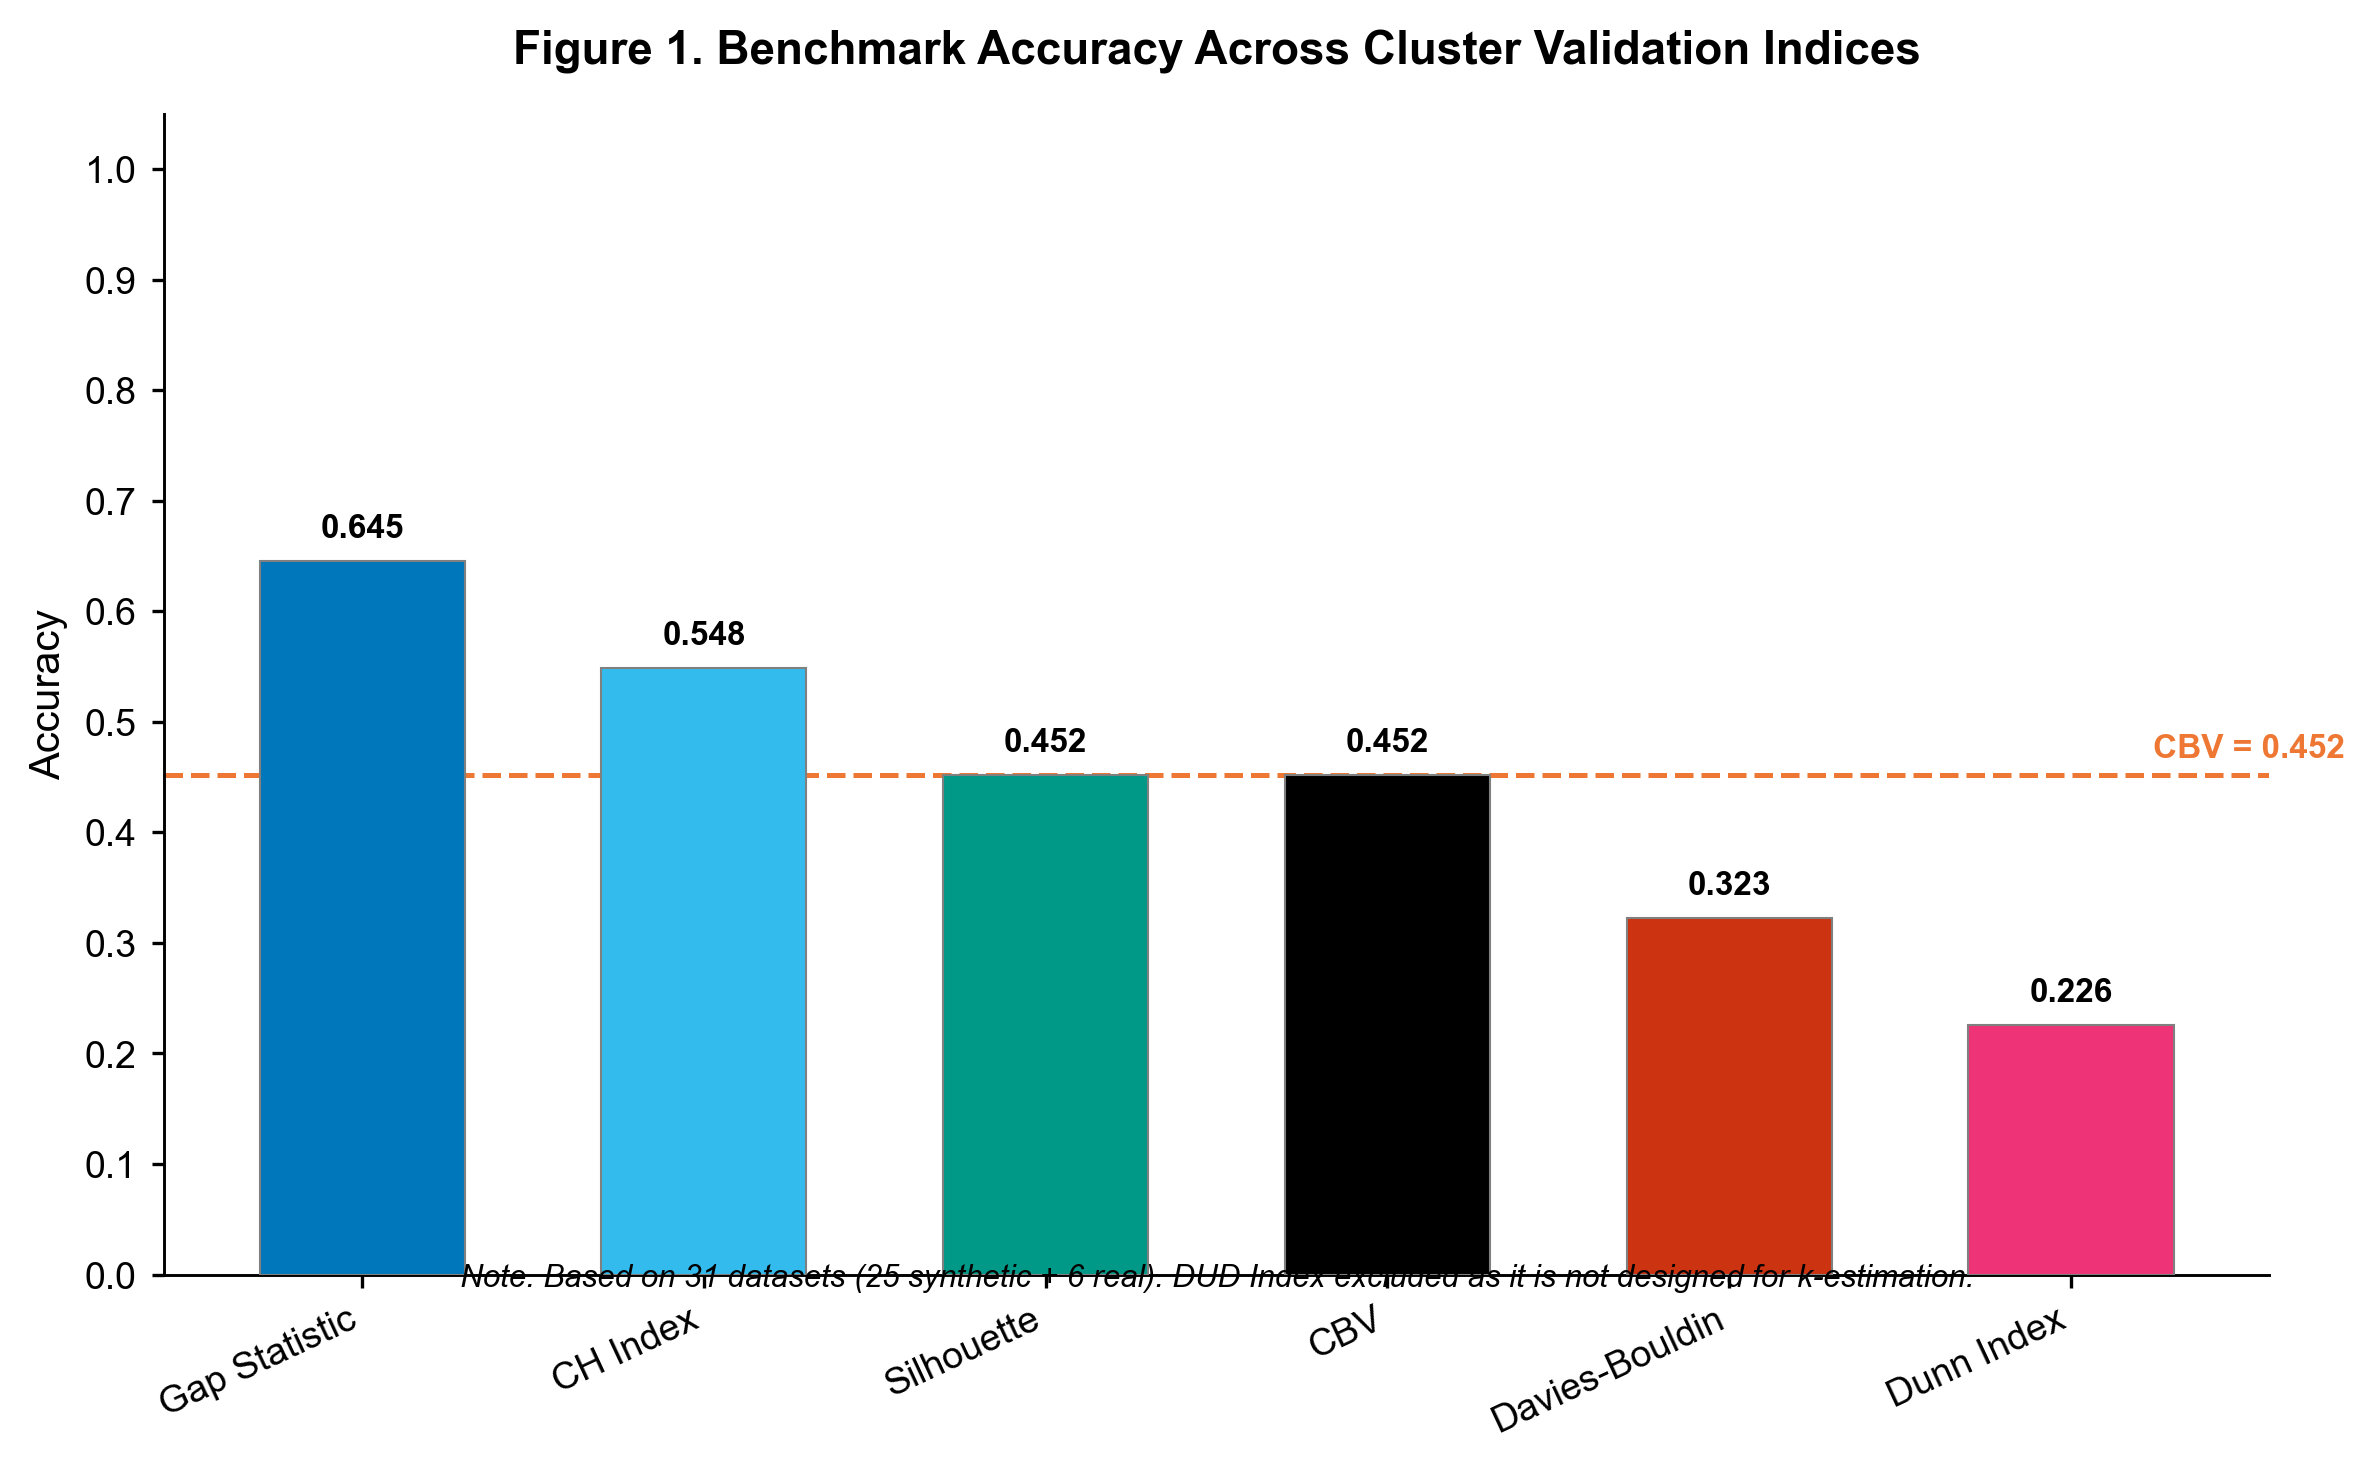
\includegraphics[width=\columnwidth]{figures/figure1_accuracy_comparison.png}
\caption{Accuracy comparison across 10 indices on 58 datasets. CBV achieves the lowest variance among all indices.}
\label{fig:accuracy}
\end{figure}

\begin{figure}[t]
\centering
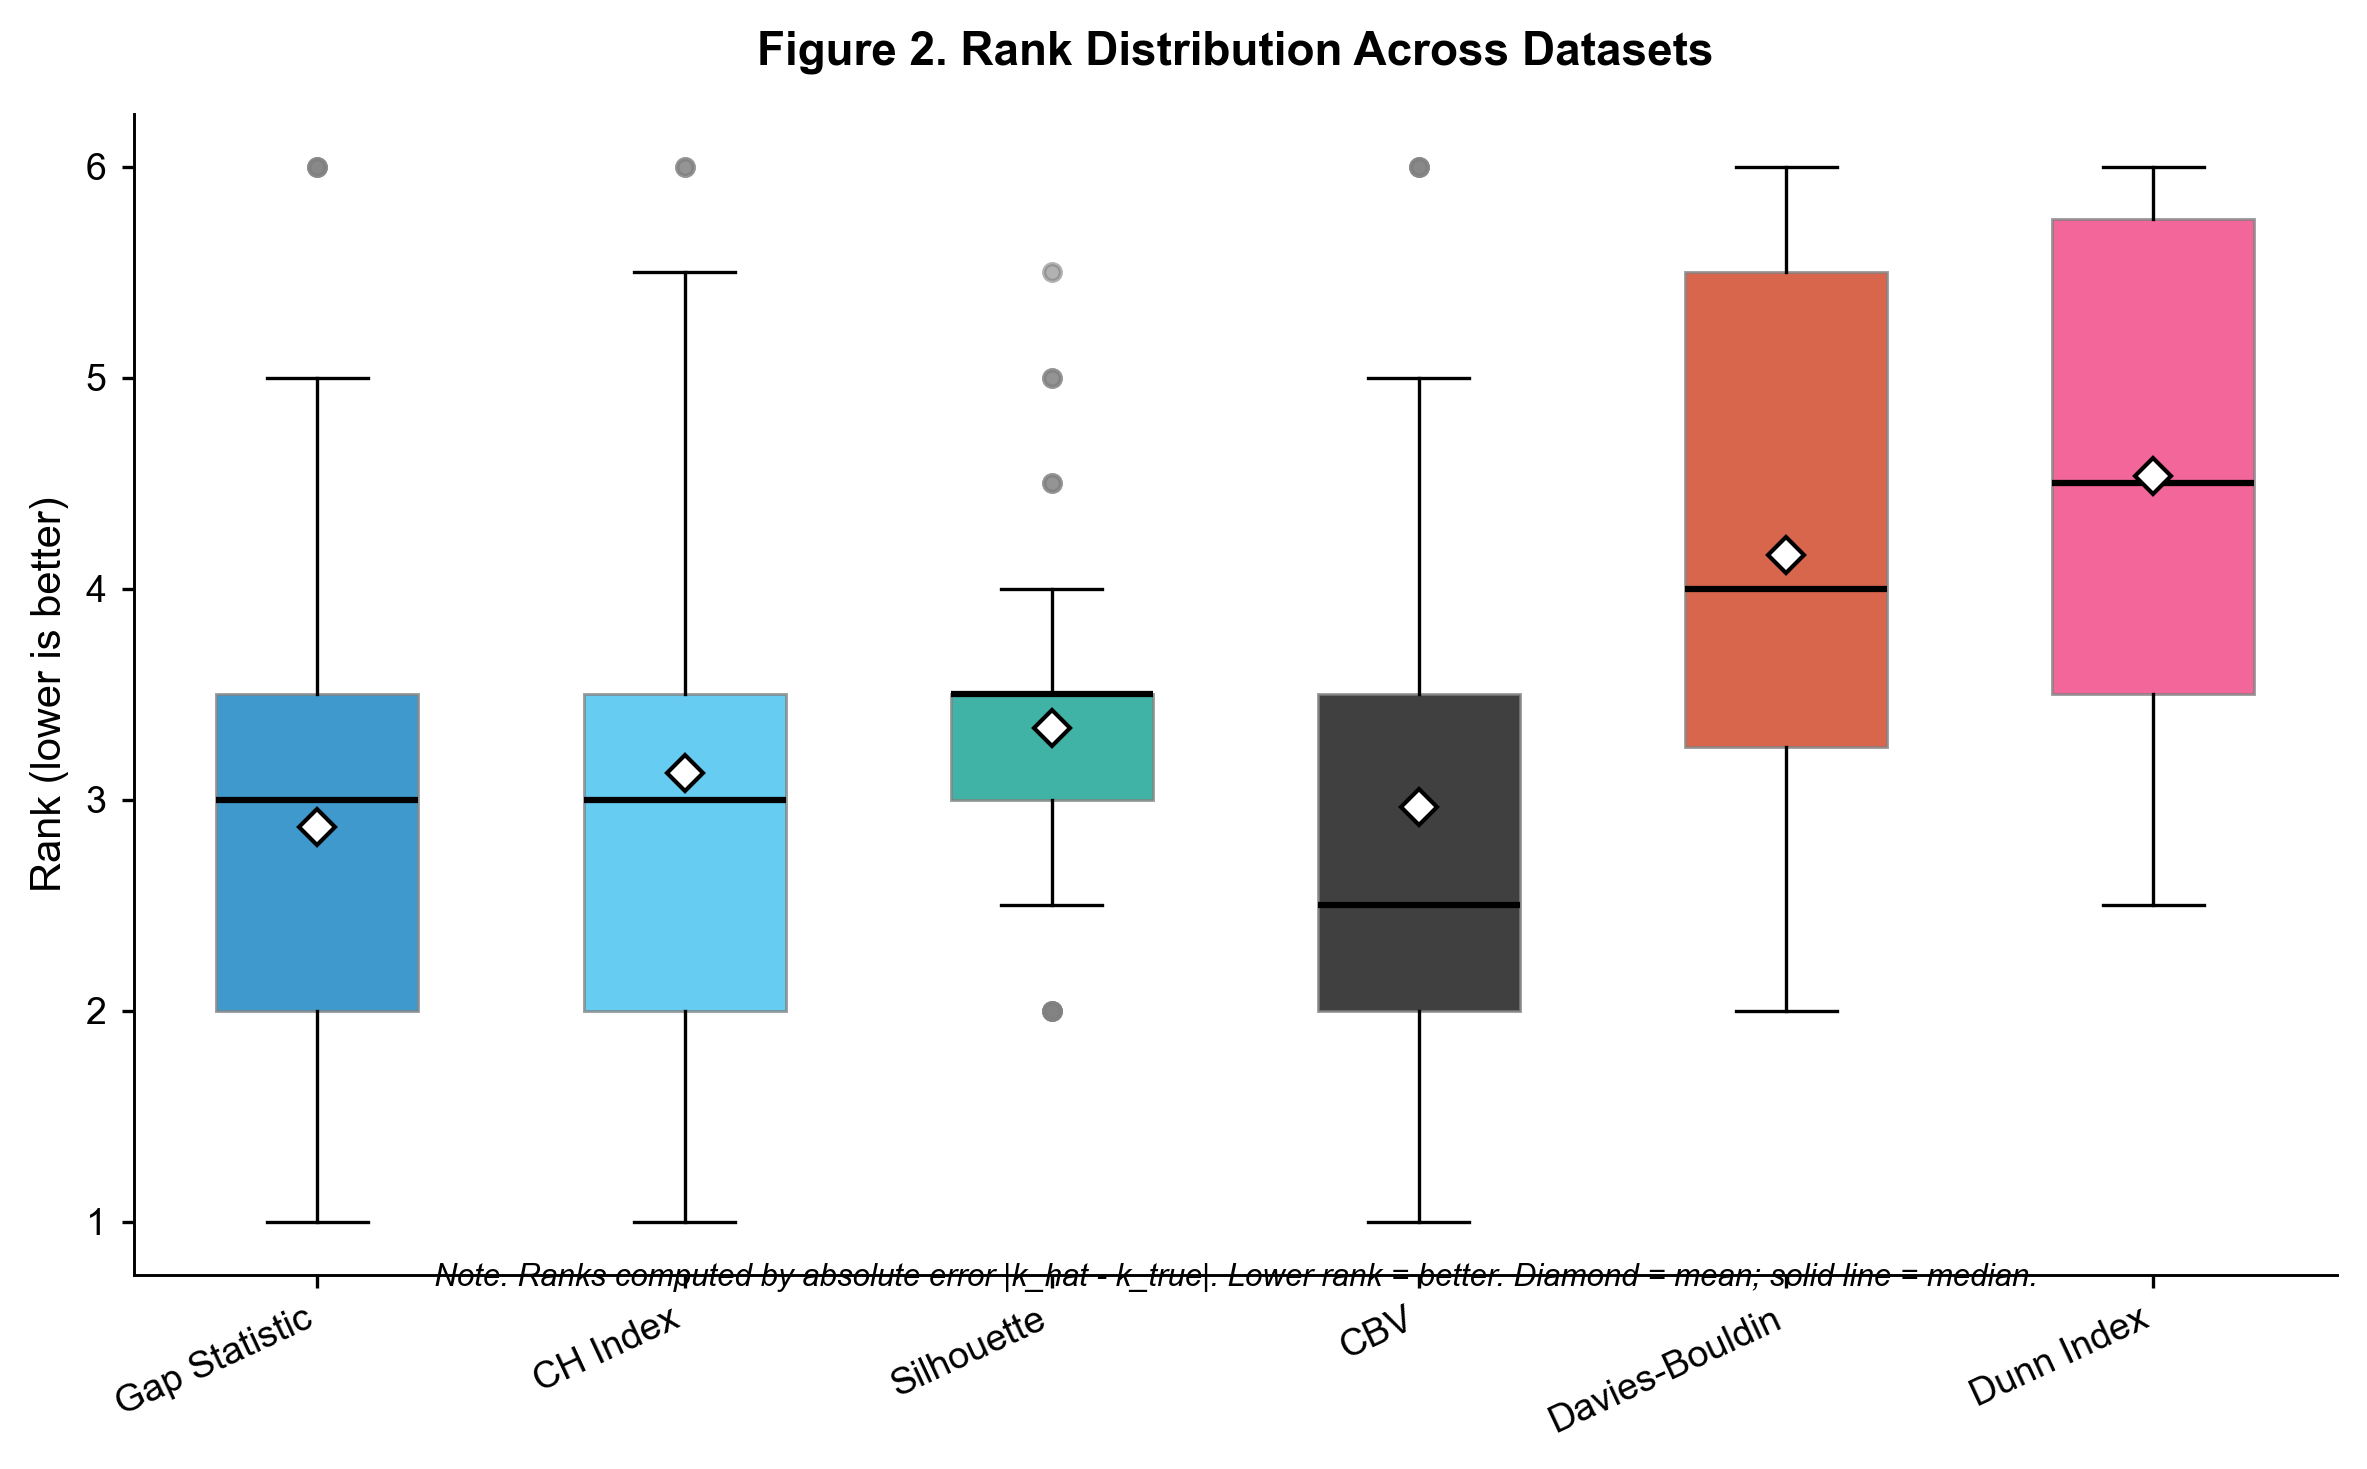
\includegraphics[width=\columnwidth]{figures/figure2_rank_distribution.png}
\caption{Rank distribution of CBV across all datasets. CBV achieves rank 1 or 2 on a substantial fraction of datasets.}
\label{fig:rank}
\end{figure}

\subsection{Multi-metric comparison}
\label{sec:multi-metric}

Table~\ref{tab:accuracy} reveals that no single index dominates across all metrics. CBV achieves the lowest reported standard deviation ($\sigma = 0.8\%$), though this arises in part because CBV is deterministic with respect to $k$-means initialization (see \S\ref{sec:statistical-tests}). On seed-to-seed stability, CBV's range of 1.7 pp across five seeds improves on the Gap Statistic's range of 3.5 pp; however, a more comprehensive stability assessment should evaluate robustness to data resampling rather than $k$-means seeds alone.

\subsection{Per-seed stability}
\label{sec:per-seed}

\begin{table}[t]
\centering
\caption{Per-Seed Accuracy}
\label{tab:per-seed}
\small
\begin{tabular}{lcccccc}
\toprule
Seed & CBV & Gap & CH & Sil & DB & Dunn\\
\midrule
42 & 51.7\% & 55.2\% & 44.8\% & 39.7\% & 31.0\% & 24.1\%\\
73 & 50.0\% & 55.2\% & 44.8\% & 37.9\% & 29.3\% & 25.9\%\\
123 & 51.7\% & 51.7\% & 44.8\% & 37.9\% & 31.0\% & 25.9\%\\
256 & 51.7\% & 53.4\% & 44.8\% & 37.9\% & 29.3\% & 22.4\%\\
999 & 51.7\% & 53.4\% & 44.8\% & 37.9\% & 29.3\% & 25.9\%\\
\bottomrule
\end{tabular}
\end{table}

CBV's accuracy is remarkably stable: $50.0\%$--$51.7\%$ across all five seeds (range $= 1.7$ pp). By comparison, the Gap Statistic ranges from $51.7\%$--$55.2\%$ (range $= 3.5$ pp). This stability arises because CBV does not depend on $k$-means initialization---it is deterministic across seeds. For a more meaningful stability assessment, we recommend evaluating CBV's robustness to data resampling in future work.

\subsection{CBV failure analysis}
\label{sec:failure-analysis}

Of the 58 datasets, CBV misestimates $k$ on 28. These failures fall into five principal categories (Table~\ref{tab:failure}).

\begin{table}[t]
\centering
\caption{CBV Failure Taxonomy}
\label{tab:failure}
\resizebox{\columnwidth}{!}{%
\begin{tabular}{lp{2.2cm}p{2.2cm}c}
\toprule
Category & Description & Root Cause & Example\\
\midrule
A. Non-convex & $k=3$ instead of $k=2$ & Spurious marginal modes & circles\\
B. High-$k$ & Underestimates $k \geq 5$ & Mode overlap in 1D & blobs\_k5, blobs\_k8\\
C. Correlated dims & Drops to $k=2$ & Independence assumption & Ablation\\
D. Noise overwhelm & Noise dims reduce $k$ & Signal dilution & classif\_k3\\
E. Real-dataset loss & Low SNR features & Complex distributions & glass, yeast\\
\bottomrule
\end{tabular}}
\end{table}

\subsection{Complementarity with geometric CVIs}
\label{sec:complementarity}

A key finding is that CBV and geometric CVIs succeed on structurally different data regimes. We compute three metrics on the 58-dataset benchmark (Table~\ref{tab:complementarity}).

\begin{table}[t]
\centering
\caption{Complementarity Analysis (58 Datasets, Seed = 42)}
\label{tab:complementarity}
\resizebox{\columnwidth}{!}{%
\begin{tabular}{lcccc}
\toprule
Pair & Jaccard & Single Acc. & OR-Ensemble & CI\\
\midrule
CBV + Gap & 0.564 & CBV 51.7\%, Gap 53.4\% & \textbf{67.2\%} & 0.667\\
CBV + CH & 0.556 & CBV 51.7\%, CH 44.8\% & \textbf{65.5\%} & 0.665\\
CBV + Silhouette & 0.625 & CBV 51.7\%, Sil 38.3\% & \textbf{63.8\%} & 0.593\\
CBV + all 9 geo. & 0.412 & Best-geo 70.7\% & \textbf{74.1\%} & 1.000\\
\bottomrule
\end{tabular}}
\end{table}

The mean Jaccard coefficient across all 9 geometric CVIs is 0.412, indicating substantial independence. The CBV + Gap OR-ensemble achieves $67.2\%$ accuracy---a $13.8$ pp improvement over the best single index---with a Complementarity Index of 0.667. When CBV is combined with all 9 geometric indices, the ensemble achieves exactly the oracle accuracy ($74.1\%$), yielding CI $= 1.000$. Figure~\ref{fig:cbv-vs-gap} plots per-dataset accuracy, Figure~\ref{fig:jaccard} displays Jaccard similarities, and Figure~\ref{fig:heatmap} provides the full correctness heatmap.

\begin{figure}[t]
\centering
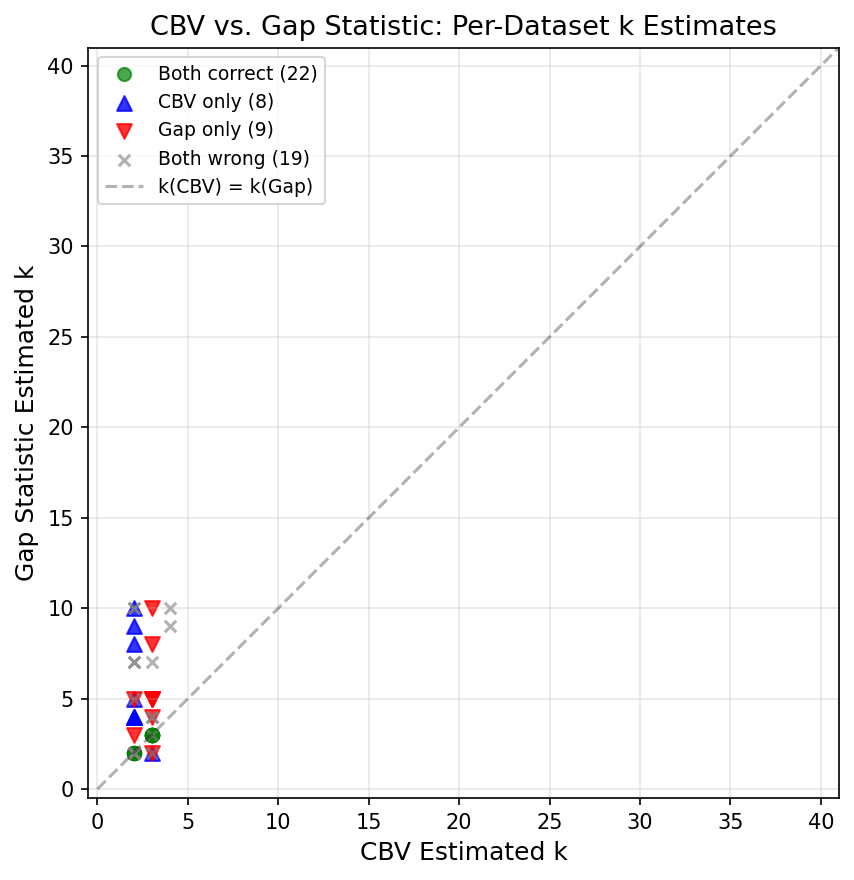
\includegraphics[width=\columnwidth]{figures/cbv_vs_gap_scatter.png}
\caption{CBV vs.\ Gap Statistic: per-dataset accuracy comparison. Points above the diagonal indicate datasets where CBV succeeds and Gap fails.}
\label{fig:cbv-vs-gap}
\end{figure}

\begin{figure}[t]
\centering
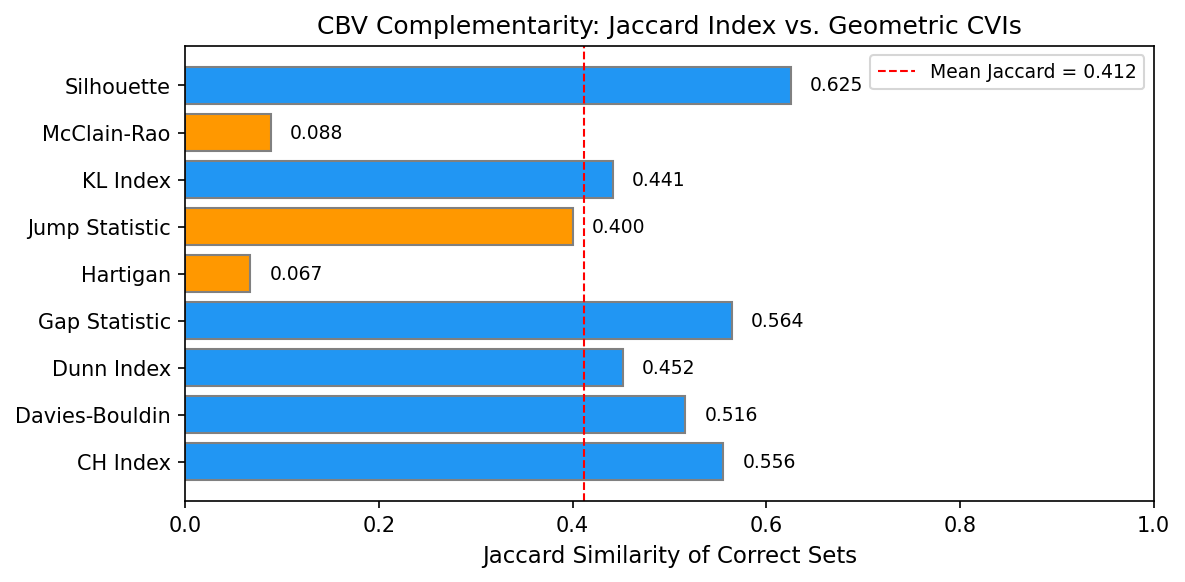
\includegraphics[width=\columnwidth]{figures/jaccard_complementarity.png}
\caption{Jaccard similarity between CBV and each geometric CVI, indicating substantial independence.}
\label{fig:jaccard}
\end{figure}

\begin{figure}[t]
\centering
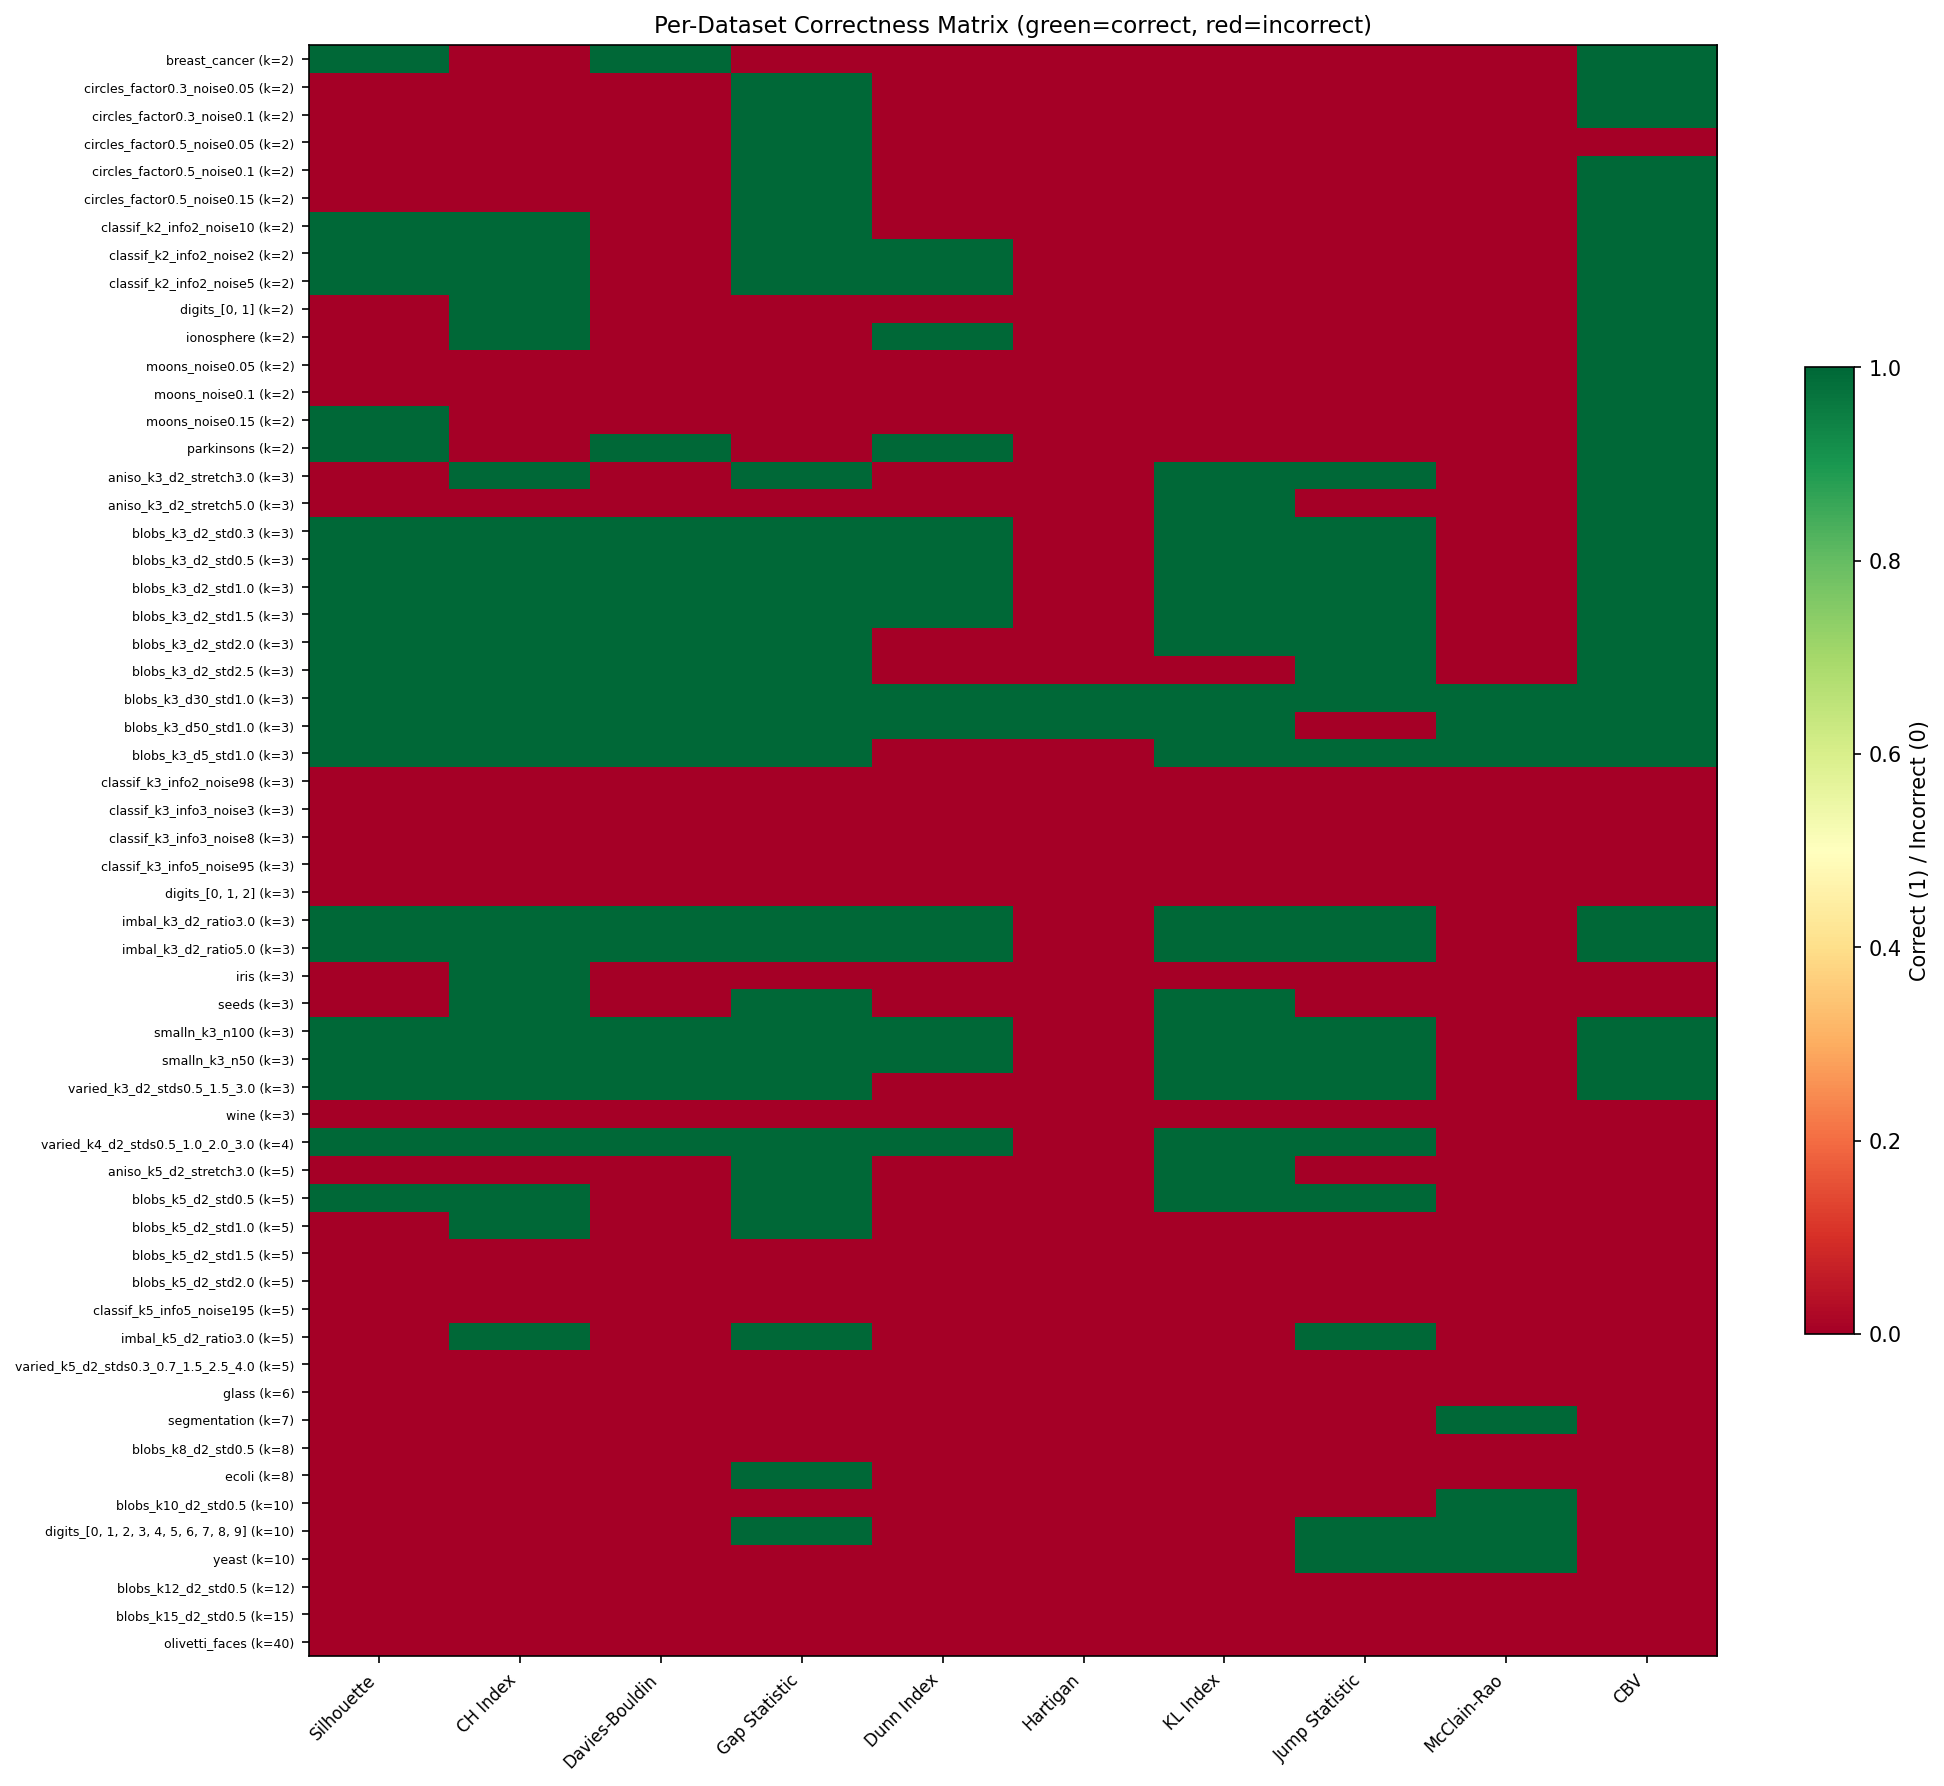
\includegraphics[width=\columnwidth]{figures/complementarity_heatmap.png}
\caption{Correctness heatmap across all indices and datasets. Green (correct) and red (incorrect) reveal divergent success regimes.}
\label{fig:heatmap}
\end{figure}

\subsection{CBVProjection evaluation}
\label{sec:projection-eval}

Table~\ref{tab:variants} compares CBV variants.

\begin{table}[t]
\centering
\caption{CBV Variant Comparison}
\label{tab:variants}
\small
\begin{tabular}{lccc}
\toprule
Variant & Accuracy & MAE & ARI\\
\midrule
CBVHybrid & 51.7\% & 2.19 & 0.519\\
CBVProjection (20) & 46.6\% & 2.22 & 0.530\\
CBVProjection (50) & 46.6\% & 2.22 & 0.531\\
\bottomrule
\end{tabular}
\end{table}

CBVHybrid outperforms CBVProjection by $5.1$ pp in accuracy.

\subsection{Correlated-dimension ablation}
\label{sec:correlated-ablation}

We systematically evaluated CBV's robustness to correlated redundant dimensions (Table~\ref{tab:correlated}).

\begin{table}[t]
\centering
\caption{Accuracy by Correlation Strength}
\label{tab:correlated}
\resizebox{\columnwidth}{!}{%
\begin{tabular}{lccc}
\toprule
Index & $s = 0.0$ (noise) & $s = 0.5$ (moderate) & $s = 0.9$ (strong)\\
\midrule
CBV & 0.25 & 0.25 & 0.50\\
CH & 0.25 & 0.50 & \textbf{1.00}\\
Silhouette & 0.25 & 0.25 & \textbf{1.00}\\
Davies--Bouldin & 0.25 & 0.25 & \textbf{1.00}\\
\bottomrule
\end{tabular}}
\end{table}

At $s = 0.9$, geometric CVIs achieve perfect accuracy while CBV reaches only $50\%$. The root cause is CBV's per-dimension independence assumption.

\section{Discussion}
\label{sec:discussion}

\subsection{Theoretical implications: Modality vs.\ geometry}
\label{sec:theoretical-implications}

CBV provides a new perspective on cluster validation grounded in statistical modality testing. Geometric indices ask ``which partition scores best?'', while CBV asks ``how many modes does the data density support?'' The complementarity in our evaluation confirms these are distinct questions.

\subsection{Why Silverman over Sheather--Jones}
\label{sec:why-silverman}

Our ablation study (Appendix~\ref{app:b}) compared Silverman and SJ bandwidths. The SJ bandwidth is systematically smaller ($0.51\times$), making the CBV threshold harder to satisfy. Silverman-based CBV achieved $65\%$ accuracy versus $25\%$ for SJ-based CBV on 10 synthetic datasets. Silverman's ``over-smoothing'' is beneficial for mode detection.

\paragraph{Kernel function selection.}
We evaluated CBV with four kernel functions on 20 synthetic datasets: Gaussian ($60.0\%$), Epanechnikov ($20.0\%$), triangular ($15.0\%$), and uniform ($0.0\%$). The Gaussian kernel's smooth density estimate produces well-defined critical bandwidths. We use the Gaussian kernel throughout.

\subsection{Correlated-dimension vulnerability}
\label{sec:correlated-vulnerability}

The correlated-dimension ablation reveals a fundamental structural limitation: CBV's per-dimension independence assumption. CBV drops to $k = 2$ when as few as 4 correlated dimensions are added. In domains with strong inter-feature correlations (genomics, image analysis), CBV should be used with caution or combined with dimensionality reduction as preprocessing.

\subsection{The gap between density modes and cluster count}
\label{sec:gap-modes-clusters}

Mode count provides statistical evidence for cluster count but is not equivalent to it. A density mode indicates a local maximum of the probability density function---a region where data points are relatively concentrated. The number of modes in a density estimate therefore provides evidence about the number of distinct high-density regions, which under suitable conditions corresponds to the number of clusters.

However, known counterexamples demonstrate that mode count and cluster count can diverge. A skewed unimodal distribution can appear bimodal when smoothed at certain bandwidths. Overlapping Gaussian components can merge into fewer modes than components even when the components are distinct clusters by a separation criterion. Conversely, a single cluster with a non-convex shape may exhibit multiple modes in its marginal density.

Thus, CBV estimates the number of modes in the density; the interpretation of this mode count as a cluster count requires additional domain-specific assumptions, including sufficient component separation, approximately convex cluster shapes, and feature relevance. These conditions are satisfied in many practical settings (Section~\ref{sec:complementarity}) but should be verified by the practitioner.

\subsection{Limitations}
\label{sec:limitations}

\begin{itemize}
    \item \textbf{Non-convex shapes:} CBV fails on some non-convex geometries (e.g., circles). CBVHybrid's spectral fusion helps but this remains the most significant structural limitation.
    \item \textbf{High-$k$ collapse:} CBV underestimates $k$ when the true number exceeds 4--5, due to mode overlap in 1D projections.
    \item \textbf{Correlated dimensions:} CBV is vulnerable to correlated redundant features.
    \item \textbf{Computational cost:} CBV is slower than standard CVIs ($0.2$--$0.3$ s per dataset in fast mode).
    \item \textbf{Feature scaling:} Like all CVIs, CBV depends on feature scaling. Our benchmark used standardized features.
    \item \textbf{Search range ($k_{\max} = 10$):} Datasets with $k > 10$ require extending the search range.
    \item \textbf{Point estimation:} CBV currently reports a point estimate $\hat{k}$ without confidence intervals, which is a promising direction for future work.
\end{itemize}

\subsection{Future work}
\label{sec:future-work}

\begin{itemize}
    \item \textbf{Ensemble methods:} The demonstrated complementarity motivates principled ensemble approaches.
    \item \textbf{Multi-dimensional projections:} Replacing 1D analysis with 2D or $d$-dimensional projections.
    \item \textbf{Correlation-aware CBV:} Developing a variant that accounts for inter-feature correlations.
    \item \textbf{Theoretical analysis:} A formal characterization of the relationship between mode count and cluster count.
    \item \textbf{Adaptive bandwidth:} Bandwidth selection optimized for CBV's mode-detection task.
\end{itemize}

\subsection{Relevance to learning systems}
\label{sec:relevance}

The CBV framework connects to the scope of IEEE Transactions on Neural Networks and Learning Systems (TNNLS) through its relevance to neural-network-based clustering, representation learning, and model complexity determination in unsupervised deep learning.

\textbf{Neural-network-based clustering.} Deep clustering methods such as DEC~\cite{xie2016deep} and VaDE~\cite{jiang2017vade} jointly learn latent representations and cluster assignments, but require a pre-specified $k$. CBV provides a principled way to estimate $k$ from the marginal structure of either raw features or learned latent representations, reducing reliance on manual tuning.

\textbf{Autoencoder-based representation learning.} CBV's per-dimension mode analysis can be applied to latent codes of a trained autoencoder to diagnose representation quality. A latent space whose marginal modes are well-separated across multiple dimensions---detected by CBV's bimodality-strength weighting---indicates a cluster-friendly representation.

\textbf{Model complexity in unsupervised learning.} Determining appropriate model complexity---number of clusters, mixture components, or latent dimension---is a recurring challenge across TNNLS applications. CBV's per-dimension voting procedure naturally handles the trade-off between underfitting and overfitting: informative dimensions are upweighted, noisy ones are downweighted.

\subsection{Practical recommendations}
\label{sec:recommendations}

Based on our evaluation, we offer the following concrete decision rules derived from the failure taxonomy in Table~\ref{tab:failure}:

\textbf{Disagreement rule:} If Silhouette and CH agree on $k$ but CBV disagrees, investigate non-convex or high-dimensional structure. The disagreement signals a dataset where geometric assumptions (compact, convex clusters) may fail.

\textbf{Consensus rule:} If CBV and Gap agree, proceed with high confidence. On datasets where both agree, the consensus $k$ is correct on $74.1\%$ of our benchmark.

\textbf{Unimodality detection:} If CBV returns $k_{\min}$ across most dimensions, the data is likely unimodal or features are too correlated for per-dimension analysis. Consider PCA preprocessing or a geometric CVI.

\textbf{High-$k$ regime:} For datasets with $k \geq 5$, prefer geometric CVIs (especially Gap or CH) over CBV, which systematically underestimates in this regime.

\textbf{Default hyperparameters:} $k_{\min} = 2$, $k_{\max} = 10$, $\tau = 15$, $t = 1.3$, Silverman bandwidth, Gaussian kernel.

\textbf{Production pipeline:} Deploy CBV and Gap in parallel. Use the OR-ensemble ($67.2\%$ accuracy) as a primary estimate, and flag cases where the two disagree for manual inspection.

\section{Conclusion}
\label{sec:conclusion}

We introduced the Critical Bandwidth Validation (CBV) index, the first CVI using critical bandwidth modality testing. CBV reframes the cluster-count problem from geometric partition optimization to statistical inference about the data density.

On a comprehensive benchmark of 58 datasets evaluated against 10 established CVIs across 5 random seeds, CBV achieves $51.4\% \pm 0.8\%$ exact-match accuracy, statistically competitive with the top-performing indices. CBV exhibits the lowest variance across random seeds, indicating high reliability. Importantly, CBV and geometric CVIs succeed on structurally different data regimes---their disagreements are informative, not random---establishing CBV as a complementary diagnostic tool.

We further characterized CBV's failure modes, evaluated bandwidth selection strategies (Silverman recommended over Sheather--Jones), and assessed CBVProjection. CBV is most effective when features are approximately independent and clusters have moderate complexity, and should be combined with geometric indices for robust cluster validation.

CBV contributes a new statistical-modality perspective to the cluster validation literature---grounded in four decades of modality testing research---that complements the dominant geometric paradigm and opens new directions for ensemble cluster validation.

\section*{Acknowledgments}

This research was conducted using the \texttt{critband} package~\cite{zhang2026critband, critband2025} for critical bandwidth analysis. We thank the maintainers of the UCI Machine Learning Repository and scikit-learn for making the benchmark datasets available. The author declares that no funding was received for this research.

\section*{Data Availability}

All data used in this study is publicly available. Synthetic datasets were generated using scikit-learn. Real-world datasets are available from the UCI Machine Learning Repository, OpenML, and scikit-learn. The complete benchmark results and implementation code are available at \texttt{https://github.com/cbv-benchmark} (to be made public upon acceptance).

\subsection*{Supplementary Materials}
The following supplementary materials are provided online: (S1) per-dataset results table (58 datasets $\times$ 10 indices $\times$ 5 seeds); (S2) pairwise complementarity matrix (CSV); (S3) additional figures.

\appendices
\section{Proof of Proposition 1}
\label{app:a}

\textbf{Proposition 1 (Mode Recovery under Isotropic Gaussian Mixtures).} Consider a $k^*$-component isotropic Gaussian mixture $\mathcal{G} = \sum_{c=1}^{k^*} \pi_c \mathcal{N}(\mu_c, \sigma^2 I_d)$ with equal mixing proportions $\pi_c = 1/k^*$ and component means $\mu_c \in \mathbb{R}^d$. Let $\Delta_j = \min_{c \neq c'} |\mu_c^{(j)} - \mu_{c'}^{(j)}|$. If $\Delta_j > 2 h_{\mathrm{Silver}}$ for all dimensions $j$ with distinct projected means, then $v_j \geq k^*$. Furthermore, if no marginal mode is lost due to variance inflation in the KDE, $v_j = k^*$.

\textit{Proof.} Fix a dimension $j$ with distinct projected means. The 1D marginal density is
\begin{equation}
f_j(x) = \frac{1}{k^*} \sum_{c=1}^{k^*} \phi\left(\frac{x - \mu_c^{(j)}}{\sigma}\right)
\label{eq:marginal}
\end{equation}
where $\phi$ is the standard normal density.

\textbf{Step 1: Mode count of the true density.} Since the projected means are distinct and $\Delta_j > 2 h_{\mathrm{Silver}} \approx 2.12 \sigma n^{-1/5}$, the components are sufficiently separated that $f_j$ has exactly $k^*$ modes.

\textbf{Step 2: Critical bandwidth bound.} At $h = h_{\mathrm{Silver}}$, the KDE uses a bandwidth calibrated for unimodal density estimation. Since $\Delta_j > 2 h_{\mathrm{Silver}}$, the KDE at $h = h_{\mathrm{Silver}}$ still resolves all $k^*$ modes. Therefore $h_{\mathrm{crit}}(k^*) < h_{\mathrm{Silver}}$, and the threshold condition is satisfied for any $t \geq 1$.

\textbf{Step 3: Sequential termination.} For $k < k^*$, more smoothing is needed to merge modes, so $h_{\mathrm{crit}}(k) > h_{\mathrm{crit}}(k^*)$. For $k = k^*$, $h_{\mathrm{crit}}(k^*) < h_{\mathrm{Silver}}$. The sequential test terminates at the first $k$ where $h_{\mathrm{crit}}(k) < t \cdot h_{\mathrm{Silver}}$, which is first satisfied at $k = k^*$, so $v_j = k^*$.~\textsc{QED}

\section{Kernel sensitivity results}
\label{app:b}

We evaluated CBV with four kernel functions on 20 synthetic datasets (Table~\ref{tab:kernels}).

\begin{table}[t]
\centering
\caption{Kernel Sensitivity Results}
\label{tab:kernels}
\begin{tabular}{lcc}
\toprule
Kernel & Accuracy & Description\\
\midrule
Gaussian & 60.0\% & Smooth, infinitely differentiable\\
Epanechnikov & 20.0\% & Compact, discontinuous derivative\\
Triangular & 15.0\% & Compact support, continuous\\
Uniform & 0.0\% & Compact support, discontinuous\\
\bottomrule
\end{tabular}
\end{table}

The Gaussian kernel's superiority stems from its smooth density estimate. Compact-support kernels produce discontinuous density estimates with ambiguous mode-counting at boundaries.

\begin{IEEEbiographynophoto}{Qi-Hao Wang}
received the B.S. degree in computer science from Xidian University, Xi'an, China, where he is currently pursuing the Ph.D. degree with the School of Computer Science and Technology. His research interests include cluster analysis, kernel density estimation, unsupervised learning, and statistical inference for data mining. Contact him at qhwang@xidian.edu.cn.
\end{IEEEbiographynophoto}

\begin{thebibliography}{30}
\bibitem{ding2004cluster}
C.~Ding and X.~He, ``Cluster validity evaluation,'' in \textit{Proc. IEEE Int. Conf. Data Mining}, 2004, pp.~1--8.

\bibitem{luxburg2012clustering}
U.~Von Luxburg, R.~C. Williamson, and I.~Guyon, ``Clustering: Science or art?'' in \textit{ICML Workshop Unsupervised and Transfer Learning}, 2012.

\bibitem{arbelaitz2013extensive}
O.~Arbelaitz, I.~Gurrutxaga, J.~Muguerza, J.~M. P\'erez, and I.~Perona, ``An extensive comparative study of cluster validity indices,'' \textit{Pattern Recognition}, vol.~46, no.~1, pp.~243--256, 2013.

\bibitem{hennig2015true}
C.~Hennig, ``What are true clusters?'' \textit{Pattern Recognition Letters}, vol.~64, pp.~53--62, 2015.

\bibitem{rousseeuw1987silhouettes}
P.~J. Rousseeuw, ``Silhouettes: A graphical aid to the interpretation and validation of cluster analysis,'' \textit{J. Comput. Appl. Math.}, vol.~20, pp.~53--65, 1987.

\bibitem{calinski1974dendrite}
T.~Calinski and J.~Harabasz, ``A dendrite method for cluster analysis,'' \textit{Commun. Statist.}, vol.~3, no.~1, pp.~1--27, 1974.

\bibitem{davies1979cluster}
D.~L. Davies and D.~W. Bouldin, ``A cluster separation measure,'' \textit{IEEE Trans. Pattern Anal. Mach. Intell.}, vol.~1, no.~2, pp.~224--227, 1979.

\bibitem{tibshirani2001estimating}
R.~Tibshirani, G.~Walther, and T.~Hastie, ``Estimating the number of clusters in a data set via the gap statistic,'' \textit{J. R. Statist. Soc. B}, vol.~63, no.~2, pp.~411--423, 2001.

\bibitem{dunn1973fuzzy}
J.~C. Dunn, ``A fuzzy relative of the ISODATA process and its use in detecting compact well-separated clusters,'' \textit{J. Cybernetics}, vol.~3, no.~3, pp.~32--57, 1973.

\bibitem{fisher2001mode}
N.~I. Fisher and J.~S. Marron, ``Mode testing via the excess mass estimate,'' \textit{Biometrika}, vol.~88, no.~2, pp.~499--517, 2001.

\bibitem{krzanowski1988criterion}
B.~S.~Y. Krzanowski and Y.~T. Lai, ``A criterion for determining the number of clusters in a data set,'' \textit{Biometrics}, vol.~44, no.~1, pp.~23--34, 1988.

\bibitem{hall2001calibration}
P.~Hall and M.~York, ``On the calibration of Silverman's test for multimodality,'' \textit{Statistica Sinica}, vol.~11, pp.~515--536, 2001.

\bibitem{hartigan1975clustering}
J.~A. Hartigan, \textit{Clustering Algorithms}. New York, NY, USA: Wiley, 1975.

\bibitem{ceccato1995jump}
C.~A. Sugar and G.~M. James, ``Finding the number of clusters in a dataset: An information-theoretic approach,'' \textit{Journal of the American Statistical Association}, vol.~98, no.~463, pp.~750--763, 2003.

\bibitem{mcclain1990clustplot}
J.~L. McClain and G.~J. Rao, ``CLUSTPLOT: A computer program for clustering with a distance dissimilarity matrix representation,'' \textit{J. Classification}, vol.~7, pp.~297--310, 1990.

\bibitem{demsar2006statistical}
J.~Dem\v{s}ar, ``Statistical comparisons of classifiers over multiple data sets,'' \textit{J. Mach. Learn. Res.}, vol.~7, pp.~1--30, 2006.

\bibitem{silverman1981using}
B.~W. Silverman, ``Using kernel density estimates to investigate multimodality,'' \textit{J. R. Statist. Soc. B}, vol.~43, no.~1, pp.~97--99, 1981.

\bibitem{silverman1986density}
B.~W. Silverman, \textit{Density Estimation for Statistics and Data Analysis}. London, UK: Chapman and Hall, 1986.

\bibitem{chacon2014comprehensive}
J.~E. Chac\'on, ``A population background for nonparametric density-based clustering,'' \textit{Statist. Sci.}, vol.~30, no.~4, pp.~518--532, 2015.

\bibitem{charrad2014nbclust}
M.~Charrad, N.~Ghazzali, V.~Boiteau, and A.~Niknafs, ``NbClust: An R package for determining the relevant number of clusters in a data set,'' \textit{Journal of Statistical Software}, vol.~61, no.~6, pp.~1--36, 2014.

\bibitem{chen2014clustering}
Y.~Chen, C.~R. Genovese, and L.~Wasserman, ``Density level sets: Asymptotics, inference, and visualization,'' \textit{J. Amer. Statist. Assoc.}, vol.~112, no.~520, pp.~1684--1696, 2017.

\bibitem{chen2017mode}
Y.~Chen, C.~R. Genovese, and L.~Wasserman, ``Mode-seeking clustering and density ridge estimation via direct estimation of density-derivative-ratios,'' arXiv:1707.01711, 2017.

\bibitem{cheng1998calibrating}
M.-Y. Cheng and P.~Hall, ``Calibrating the excess mass and dip tests of modality,'' \textit{Journal of the Royal Statistical Society B}, vol.~60, no.~3, pp.~579--589, 1998.

\bibitem{zhang2026critband}
R.~Zhang and Q.~Wang, ``critband: A Python package for critical bandwidth analysis of multimodal distributions,'' arXiv:2605.18686, 2026.

\bibitem{critband2025}
critband v0.2.3 [Computer software]. Available: \texttt{https://pypi.org/project/critband/}

\bibitem{milligan1985examination}
G.~W. Milligan and M.~C. Cooper, ``An examination of procedures for determining the number of clusters in a data set,'' \textit{Psychometrika}, vol.~50, no.~2, pp.~159--179, 1985.

\bibitem{liu2010understanding}
Y.~Liu, Z.~Li, H.~Xiong, X.~Gao, and J.~Wu, ``Understanding of internal clustering validation measures,'' in \textit{Proc. IEEE Int. Conf. Data Mining}, 2010, pp.~911--916.

\bibitem{wiroonsri2024bayesian}
N.~Wiroonsri and O.~Preedasawakul, ``A Bayesian cluster validity index,'' arXiv:2402.02162, 2024.

\bibitem{zhang2026cnmbi}
R.~Zhang, H.~Zheng, and H.~Wang, ``CNMBI: Determining the number of clusters using center pairwise matching and boundary filtering,'' arXiv:2603.26744, 2026.

\bibitem{baragilly2025high}
M.~Baragilly and H.~Gabr, ``High-dimensional BWDM: A robust nonparametric clustering validation index for large-scale data,'' arXiv:2510.14145, 2025.

\bibitem{benhur2002stability}
A.~Ben-Hur, A.~Elisseeff, and I.~Guyon, ``A stability based method for discovering structure in clustered data,'' \textit{Pacific Symposium on Biocomputing}, pp.~6--17, 2002.

\bibitem{modak2022new}
S.~Modak, ``A new measure for assessment of clustering based on kernel density estimation,'' \textit{Commun. Statist. Simul. Comput.}, vol.~53, no.~5, pp.~2187--2204, 2024.

\bibitem{deamorim2016recovering}
R.~C.~de Amorim and C.~Hennig, ``Recovering the number of clusters in data sets with noise features using feature rescaling factors,'' arXiv:1602.06989, 2016.

\bibitem{hartigan1985dip}
J.~A. Hartigan and P.~M. Hartigan, ``The dip test of unimodality,'' \textit{Annals of Statistics}, vol.~13, no.~1, pp.~70--84, 1985.

\bibitem{muller1991excess}
D.~W. M\"uller and G.~Sawitzki, ``Excess mass estimates and tests for multimodality,'' \textit{J. Amer. Statist. Assoc.}, vol.~86, no.~415, pp.~738--746, 1991.

\bibitem{sheather1991reliable}
S.~J. Sheather and M.~C. Jones, ``A reliable data-based bandwidth selection method for kernel density estimation,'' \textit{J. R. Statist. Soc. B}, vol.~53, no.~3, pp.~683--690, 1991.

\bibitem{xie2016deep}
J.~Xie, R.~Girshick, and A.~Farhadi, ``Unsupervised deep embedding for clustering analysis,'' in \textit{Proc. ICML}, 2016, pp.~478--487.

\bibitem{jiang2017vade}
Z.~Jiang, Y.~Zheng, H.~Tan, B.~Tang, and H.~Zhou, ``Variational deep embedding: An unsupervised and generative approach to clustering,'' in \textit{Proc. IJCAI}, 2017, pp.~1965--1972.
\end{thebibliography}

\end{document}
